% master.tex : master file for the project
% ------------------------------------------------------------------------------
% This is the main file in the project, which collects the contents from all the
% input files (text, images, literature databases, etc.).

% The 'book' class is a document class with many flexible options.
% See https://tex.stackexchange.com/a/36989/118167
\documentclass[11pt,a4paper,twoside,openright,english]{book}

% Some top level variables that are used to automatically input title, authors,
% etc. in the title page and front page.
\def \projecttitle       {Empirical Financial Modelling and Applied Econometrics}
\def \projectsubtitle    {VIX and stuff}
\def \projecttheme       {Project Theme}
\def \projectdegree      {Mathematics-Economics}  % or Mathematics-Economics/Technology
\def \projectperiod      {Fall Semester 2021}
\def \projectnumber      {P7}
\def \projectgroup       {5.230b}
\def \projectauthors     {
  Christian Bang Jensen\\
  Houssam Al-Hanafi\\
  % ...
}
\def \projectsupervisors {
  Orimar Sauri\\
  % ...
}

% The preamble, i.e. all the settings and commands that go before actual
% document contents, in this template is handled in the single file aaumath.sty,
% which defines a package that can be loaded here with \usepackage.
\usepackage{aaumath}

% All contents of the document go between the \begin and \end commands for the
% 'document' environment.
\begin{document}

% The front matter is not counted in the numbered pages and are instead numbered
% with roman numerals. This consists of, for example, the front page, title
% page, preface, and table of contents.
\frontmatter
% incl/misc/frontpage.tex : document front page
% ------------------------------------------------------------------------------


\backgroundsetup{
  scale = 1,
  angle=0,
  opacity=1,
  contents = {
    
\includegraphics[width=\paperwidth,height=\paperheight]{fig/img/aau/waves.pdf}
  }
}
\BgThispage
\pdfbookmark[0]{Front page}{frontpage}
\begin{titlepage}
  \centering
  \phantom{}
  \vspace{2cm}

  % AAU badge
  \begin{minipage}[c]{0.2\paperwidth}
    \centering
    \makebox[0pt]{
      % fig/tikz/aau-badge.tex : AAU logo badge for the front page
% ------------------------------------------------------------------------------

\begin{tikzpicture}
  % Draw white circle and add the transparent blue logo on top
  \node[circle,color=white,fill=white,minimum size=1.175\textwidth] at (0,0) {};
  \node at (0,0) {
\includegraphics[width=\textwidth]{fig/img/aau/logo-circle.pdf}};
\end{tikzpicture}

    }
  \end{minipage}

  % Main contents
  \vspace{4cm}
  {\fontfamily{bch}\selectfont
    \fboxsep0pt\colorbox{white}{
      \begin{minipage}{\textwidth}
        \centering
        \color{AAUblue1}

        \vspace{2em}
        {\Huge\bfseries\projecttitle}

        {\Large\bfseries\projectsubtitle}

        \bigskip
        \parbox{\textwidth}{\centering\large\projectauthors}

        \bigskip
        {\bfseries\large{\projectnumber} Project, Group \projectgroup, \projectdegree}
        \vspace{2em}
      \end{minipage}
    }
  }

\end{titlepage}

% incl/misc/titlepage.tex : project title page
% ------------------------------------------------------------------------------
% The title page is generated by the command \aautitlepage, which is defined in
% /incl/pre/ext/aautitlepage.sty


\pdfbookmark[0]{Title page}{titlepage}
\aautitlepage{
  \projectinfo{
    \projecttitle
  }{
    \projecttheme
  }{
    \projectperiod
  }{
    Group \projectgroup
  }{
    \parbox[t]{\textwidth}{\projectauthors}
  }{
    \parbox[t]{\textwidth}{\projectsupervisors}
  }{
    \today
  }
}{
  \textbf{Dept. of Mathematical Sciences}\\
  Skjernvej 4A\\
  DK-9220 Aalborg Ø\\
  \href{http://math.aau.dk}{http://math.aau.dk}
}{
  % incl/misc/abstract.tex : project abstract
% ------------------------------------------------------------------------------
% The abstract is a short summary of the document, displayed on the title page

}

% incl/misc/contents.tex :
% ------------------------------------------------------------------------------

\pdfbookmark[0]{Contents}{contents}

% The settings in this file are grouped so they only apply here
\begingroup

% Temporarily disable twoside layout to avoid blank pages in this section
\makeatletter
\@twosidefalse
\makeatother

% Put table of contents on its own page (best for a TOC that fits on one page)
\tableofcontents
\clearpage

% Put the lists on subsequent pages without page breaks
\let\clearpage\relax
\listoffigures
\listoftables
\listofalgorithms
\lstlistoflistings

\endgroup


% The main matter is were the bulk of your work goes. Pages and headings have
% arabic numbers.
\mainmatter

%\chapter{Mathematical Prerequisites}
\section{Fundamental Definitions}
This section is based on 123...

\begin{defn}[\textit{Measurable Map, Random Element, Random Variable}]
Let $(\Omega,\mathcal{F})$ and $(\Gamma,\mathcal{G})$ be two measurable spaces. Then any map $f:\Omega\to\Gamma$ is said to be $\mathcal{F}$-$\mathcal{G}$-measurable iff $f^{-1}(E)\in\mathcal{F}$ for all $E\in\mathcal{G}$. If there is a probability measure on $(\Omega,\mathcal{F})$ present in the discussion, then any $\mathcal{F}$-$\mathcal{G}$-measurable map is called a random element and every real valued $\mathcal{F}$-$\mathcal{B}(\R)$-measurable map is called a random variable.
\end{defn}
Note that a map will simply be referred to as measurable if the concerned $\sigma$-algebras are clear from the context.

%A convenient property of measurable maps is introduced below.
%\begin{prop}\label{prop:fdr1}
%Let $(\Omega,\mathcal{F})$ and $(\R,\mathcal{B}(\R))$ be two measurable spaces. Assume that $f:\Omega\to\R$ is measurable, and that $g:\R\to\R$ is continuous. Then $g\circ f:\Omega\to\R$ is a measurable map. 
%\end{prop}
%The proof of this assertion is omitted since it follows from more general results. The interested reader is referred to the references listed at the beginning of this section.

%\begin{prop}\label{prop:fdr1}
%Let $(\Omega,\mathcal{F})$ be a measurable space, and let $(\Sigma,d_{\Sigma})$ and $(\Upsilon,d_{\Upsilon})$ be two metric spaces. Assume that $f:\Omega\to\Sigma$ is $\mathcal{F}$-$\mathcal{B}(\Sigma)$-measurable, and that $g:\Sigma\to\Upsilon$ is continuous. Then $g\circ f:\Omega\to\Upsilon$ is $\mathcal{F}$-$\mathcal{B}(\Upsilon)$-measurable.
%\end{prop}
%\begin{proof}
%\end{proof}
%As per the next result, linear combinations and products of measurable functions are again measurable.
%\begin{prop}\label{eq:fdr3}
%Let $(\Omega,\mathcal{F})$ be a measurable space. Assume that $f_{i}:\Omega\to\R$ is $\mathcal{F}$-$\mathcal{B}(\R)$-measurable for every $i\in\{1,\dots,n\}$ with $n\in\N$, and that $P:\R^{n}\to\R$ is some polynomial. Then the map $g:\Omega\to\R$ defined by:
%\begin{equation}
%    g(\omega)\coloneqq P(f_{1}(\omega),\dots,f_{n}(\omega)),\quad\omega\in\Omega,
%\end{equation}
%is $\mathcal{F}$-$\mathcal{B}(\R)$-measurable.
%\end{prop}
%\begin{proof}
%\end{proof}

%\begin{prop}
%Let $(\Omega,\mathcal{F})$, $(\Gamma,\mathcal{G})$, and $(\Sigma,\mathcal{Q})$ be three measurable spaces. Assume that $f:\Omega\to\Gamma$ is $\mathcal{F}$-$\mathcal{G}$-measurable, and that $g:\Gamma\to\Sigma$ is $\mathcal{G}$-$\mathcal{Q}$-measurable. Then $g\circ f:\Omega\to\Sigma$ is $\mathcal{F}$-$\mathcal{Q}$-measurable. Moreover 
%\end{prop}
%\begin{proof}
%Let $A\in\mathcal{Q}$. Then it immediately follows from the the measurability of $g$ and $f$ that:
%\begin{equation*}
%    (g\circ f)^{-1}(A)=f^{-1}(g^{-1}(A))\in\mathcal{F}.\qedhere
%\end{equation*}
%\end{proof}

\begin{defn}[\textit{Stochastic Process}]
Let $(\Omega,\mathcal{F},\mathbb{P})$ be a probability space, $(\Gamma,\mathcal{G})$ a measurable space, and $I\subseteq\R$ be non-empty. Then a family $X=(X_{t})_{t\in I}$ of random elements $X_{t}:\Omega\to\Gamma$ is called a stochastic process on $(\Omega,\mathcal{F},\mathbb{P})$ with target space $(\Gamma,\mathcal{G})$ and index set $I$. %If $I$ is countable, then $X$ is called discrete.
\end{defn}
Note that, in this project report, it is henceforth assumed, unless specified otherwise, that any stochastic process is defined on a probability space $(\Omega,\mathcal{F},\mathbb{P})$  with target space $(\R,\mathcal{B}(\R))$ and index set $\Z$. The term time series is often used synonymously for a stochastic process of the aforementioned form.
\begin{defn}[\textit{Path Map, Sample Path}]\label{defn:pmsm}
Let $X=(X_{t})_{t\in I}$ be a stochastic process on the probability space $(\Omega,\mathcal{F},\mathbb{P})$ with target space $(\Gamma,\mathcal{G})$. Then the path map $X_{\bullet}:\Omega\to\Gamma^{I}$ associated with $X$ is defined as:
\begin{equation}
    (X_{\bullet}(\omega))(t)\coloneqq X_{t}(\omega),\quad\omega\in\Omega,\, t\in I.
\end{equation}
Moreover, the image point $X_{\bullet}(\omega)\in\Gamma^{I}$ is called the sample path corresponding to $\omega\in\Omega$.
\end{defn}
Note that in Definition \ref{defn:pmsm}, the notation $\Gamma^{I}$ denotes the set of all maps from $I$ to $\Gamma$.
\begin{defn}[\textit{Filtration}]
Let $(\Omega,\mathcal{F})$ be a measurable space. Then a family $(\mathcal{F}_{t})_{t\in\Z}$ of sub-$\sigma$-algebras of $\mathcal{F}$ such that $\mathcal{F}_{s}\subseteq\mathcal{F}_{t}\subseteq\mathcal{F}$ for all $s,t\in\Z$ with $s\leq t$ is called a filtration on $(\Omega,\mathcal{F})$. 
\end{defn}
\begin{defn}[\textit{Adapted Process}]
Let $X=(X_{t})_{t\in\Z}$ be a stochastic process on the probability space $(\Omega,\mathcal{F},\mathbb{P})$ with target space $(\Gamma,\mathcal{G})$, and let $(\mathcal{F}_{t})_{t\in\Z}$ be a filtration on $(\Omega,\mathcal{F})$. Then $X$ is called adapted to $(\mathcal{F}_{t})_{t\in\Z}$ iff $X_{t}:\Omega\to\Gamma$ is $\mathcal{F}_{t}$-measurable for all $t\in\Z$.
\end{defn}
Note that a stochastic process will simply be referred to as adapted if the filtration is clear from the context.
\begin{defn}[\textit{Natural Filtration}]\label{defn:naturalfiltration}
Let $X=(X_{t})_{t\in\Z}$ be a stochastic process on the probability space $(\Omega,\mathcal{F},\mathbb{P})$ with target space $(\Gamma,\mathcal{G})$. Then the natural filtration associated with $X$ is defined as:
\begin{equation}
    \mathcal{F}_{t}^{X}\coloneqq\sigma\left(\left\{X_{s}^{-1}(E)\mid E\in\mathcal{G},\hspace{4pt} s\in(-\infty,t]\cap\Z\right\}\right),\quad t\in\Z.
\end{equation}
\end{defn}
Note that a stochastic process is by definition adapted to its natural filtration.
\begin{defn}[\textit{Independence}]\label{defn:ind}
Let $(\Omega,\mathcal{F},\mathbb{P})$ be a probability space. Then $\mathcal{M}_{1},\dots,\mathcal{M}_{n}\subseteq\mathcal{F}$ are called independent iff for every non-empty $J\subseteq\{1,\dots,n\}$ with $n\in\N$, it holds that:
\begin{equation}
    \mathbb{P}\left(\hspace{2pt}\bigcap\limits_{i\in J}A_{i}\right)=\prod_{i\in J}\mathbb{P}(A_{i}),\quad A_{i}\in\mathcal{M}_{i}.
\end{equation}
The events $A_{1},\dots,A_{n}\in\mathcal{F}$ are called independent iff $\{A_{1}\},\dots,\{A_{n}\}\subseteq\mathcal{F}$ are independent. Moreover, let $(\Gamma_{i},\mathcal{G}_{i})$ be measurable spaces, and let $X_{i}:\Omega\to\Gamma_{i}$ be random elements for every $i\in\{1,\dots,n\}$. Then $X_{1},\dots,X_{n}$ are called independent iff their induced $\sigma$-algebras, $\sigma(X_{1}),\dots,\sigma(X_{n})$, are independent.
\end{defn}
Note that in Definition \ref{defn:ind}, the $\sigma$-algebra induced by $X_{i}$ is defined as:
\begin{equation}
    \sigma(X_{i})\coloneqq X_{i}^{-1}(\mathcal{G}_{i})\coloneqq\{X_{i}^{-1}(E_{i})\mid E_{i}\in\mathcal{G}_{i}\}.
\end{equation}
%\begin{prop}\label{prop:fdr2}
%Let $(\Omega,\mathcal{F},\mathbb{P})$ be a probability space, and let $(\Gamma_{i},\mathcal{G}_{i})$ and $(\Sigma_{i},\mathcal{Q}_{i})$ be measurable spaces for every $i\in\{1,\dots,n\}$ with $n\in\N$. Assume that $X_{i}:\Omega\to\Gamma_{i}$ are random elements, and that $F_{i}:\Omega_{i}\to\Sigma_{i}$ is a measurable map for every $i\in\{1,\dots,n\}$. If $X_{1},\dots,X_{n}$ are independent, then $F_{1}\circ X_{1},\dots,F_{n}\circ X_{n}$ are again independent.
%\end{prop}
%Note that the previous result can be generalized to hold for a composition of a continuous map with a random element, cf. Proposition \ref{prop:fdr1}.
%\begin{proof}
%This result immediately follows by noticing that the $\sigma$-algebra induced by $F_{i}\circ X_{i}$ is smaller than the $\sigma$-algebra induced by $X_{i}$ for every $i\in\{1,\dots,n\}$.
%\end{proof}
\begin{defn}[\textit{Independent Increments}]
Let $X=(X_{t})_{t\in I}$ be a stochastic process on $(\Omega,\mathcal{F},\mathbb{P})$ with target space $(\R^{d},\mathcal{B}(\R^{d}))$. Then $X$ is said to be a process with independent increments iff its increments:
\begin{equation}
    X_{0},\quad X_{t_{1}}-X_{0},\quad\dots,\quad X_{t_{n}}-X_{t_{n-1}},
\end{equation}
are independent for all $n\in\N$ and $t_{1},\dots,t_{n}\in I$ with $0<t_{1}<\dots<t_{n}$.
\end{defn}
\begin{defn}[\textit{Expectation}]
Let $(\Omega,\mathcal{F},\mathbb{P})$ be a probability space, and let $f:\Omega\to\R$ be $\mathbb{P}$-integrable function. Then the expectation of $f$ is defined as:
\begin{equation}
    \mathbb{E}[f]\coloneqq\int_{\Omega}f\,\mathrm{d}\mathbb{P}.
\end{equation}
\end{defn}
\begin{defn}[\textit{Kurtosis, Leptokurticity}\textcolor{red}{*}]\label{defn:kurtosis}
Let $(\Omega,\mathcal{F},\mathbb{P})$ be a probability space, and let $f:\Omega\to\R$ with $\mathbb{E}[f^{4}]<\infty$. Then the kurtosis of $f$ is defined as:
\begin{equation}
    \kappa(f)\coloneqq\frac{\mathbb{E}[(f-\mathbb{E}[f])^{4}]}{\left(\mathbb{E}\left[(f-\mathbb{E}[f])^{2}\right]\right)^{2}}.
\end{equation}
\end{defn}
\begin{defn}[\textit{Conditional Expectation}]
Let $(\Omega,\mathcal{F},\mathbb{P})$ be a probability space, $\mathcal{A}\subseteq\mathcal{F}$ a sub-$\sigma$-algebra, and $f:\Omega\to\R$ a $\mathbb{P}$-integrable function. Then a function $g:\Omega\to\R$ is called a representative of the conditional expectation of $f$ under the hypothesis $\mathcal{A}$ iff it is $\mathbb{P}$-integrable, $\mathcal{A}$-measurable, and:
\begin{equation}
    \int_{A}f\,\mathrm{d}\mathbb{P}=\int_{A}g\,\mathrm{d}\mathbb{P},\quad A\in\mathcal{A}.
\end{equation}
\end{defn}
123123

\begin{thm}
Let $(\Omega,\mathcal{F},\mathbb{P})$ be a probability space, $\mathcal{A}\subseteq\mathcal{F}$ a sub-$\sigma$-algebra, and $f:\Omega\to\R$ a $\mathbb{P}$-integrable function. Then:
\begin{enumerate}[label=(\roman*)]
\item Linearity: Let $g:\Omega\to\R$ be $\mathbb{P}$-integrable, and let $\alpha,\beta\in\R$. Then:
\begin{equation}\label{eq:celin}
    \mathbb{E}[\alpha f +\beta g\mid\mathcal{A}]=\alpha\mathbb{E}[f\mid\mathcal{A}]+\beta\mathbb{E}[g\mid\mathcal{A}],\quad\textrm{$\mathbb{P}$-a.s.}
\end{equation}
\item Tower property: If $\mathcal{B}\subseteq\mathcal{F}$ is another sub-$\sigma$-algebra such that $\mathcal{A}\subseteq\mathcal{B}$, then:
\begin{equation}\label{eq:cetp}
    \mathbb{E}[\mathbb{E}[f\mid\mathcal{B}]\mid\mathcal{A}]=\mathbb{E}[\mathbb{E}[f\mid\mathcal{A}]\mid\mathcal{B}]=\mathbb{E}[f\mid\mathcal{A}],\quad\textrm{$\mathbb{P}$-a.s.}
\end{equation}
\item Pull-out property: Let $g:\Omega\to\R$ be $\mathcal{A}$-measurable. Then $fg$ is $\mathbb{P}$-integrable iff $g\mathbb{E}[f\mid\mathcal{A}]$ is $\mathbb{P}$-integrable, and:
\begin{equation}\label{eq:cepop}
    \mathbb{E}[fg\mid\mathcal{A}]=g\mathbb{E}[f\mid\mathcal{A}],\quad\textrm{$\mathbb{P}$-a.s.}
\end{equation}
\item If the $\sigma$-algebra induced by $f$ and $\mathcal{A}$ are independent, then
\begin{equation}\label{eq:ceind}
    \mathbb{E}[f\mid\mathcal{A}]=\mathbb{E}[f],\quad\textrm{$\mathbb{P}$-a.s.}
\end{equation}
\item Jensen's inequality: Let $\varphi:\R\to\R$ be convex, and assume that $\varphi\circ f:\Omega\to\R$ is $\mathbb{P}$-integrable. Then:
\begin{equation}\label{eq:cejens}
    \varphi\left(\mathbb{E}[f\mid\mathcal{A}]\right)\leq\mathbb{E}[\varphi(f)\mid\mathcal{A}],\quad\textrm{$\mathbb{P}$-a.s.}
\end{equation}
\end{enumerate}
\end{thm}
%For a proof the interested reader is referred to \ref{}.

\begin{defn}[\textit{Cumulative Distribution Function}]
Let $(\Omega,\mathcal{F},\mathbb{P})$ be a probability space, and let $t=(t_{1},\dots,t_{n})\in\Z^{n}$ for $n\in\N$ with $t_{1}<\dots<t_{n}$. Suppose that $X_{t}=(X_{t_{1}},\dots,X_{t_{n}}):\Omega\to\R_{n}$ is a random vector. Then the cumulative distribution function $F_{t}:\R^{n}\to[0,1]$ of $X_{t}$ is defined as:
\begin{equation}
    F_{t}(x)\coloneqq\mathbb{P}\left(\bigcap\limits_{i=1}^{n}\{\omega\in\Omega\mid X_{t_{i}}\leq x_{i}\}\right),\quad x=(x_{1},\dots,x_{n})\in\R^{n}.
\end{equation}
\end{defn}
%In order to introduce the concept of strict stationarity, recall that if $t=(t_{1},t_{2},\dots,t_{n})\in\Z^{n}$ is an ordered tuple of integers, then the distribution function $F_{t}:\R^{n}\to [0,1]$ of a random vector $X_{t}=(X_{t_{1}},X_{t_{2}},\dots, X_{t_{n}}): (\Omega,\mathcal{F},\mathbb{P})\to (\R^{n},\mathcal{B}(\R^{n}))$ is then given by
%\begin{equation}
%    F_{t}(x)=\mathbb{P}\left(\bigcap_{i=1}^{n}\left\{\omega\in\Omega\mid X_{t_{i}}(\omega)\leq x_{i}\right\}\right),\quad x=(x_{1},x_{2},\dots,x_{n})\in\R^{n}.
%\end{equation}
\begin{defn}[\textit{Strict, Weak Stationarity}]
Let $X=(X_{t})_{t\in\Z}$ be a stochastic process. Then $X$ is said to be strictly stationary iff: %for all $n\in\N$, $t_{1},\dots,t_{n}\in\Z$ with $t_{1}<\dots<t_{n}$, and $h\in\Z$, it holds that:
\begin{equation}
    F_{(t_{1},\dots,t_{n})}=F_{(t_{1+h},\dots,t_{n+h})},
\end{equation}
for all $n\in\N$, $t_{1},\dots,t_{n}\in\Z$ with $t_{1}<\dots<t_{n}$, and $h\in\Z$. Moreover, $X$ is said to be weakly stationary iff for all $t,s,h\in\Z$, it holds that:
\begin{equation*}
    \textrm{(i)}\hspace{6pt}\mathbb{E}[X_{t}^{2}]<\infty,\qquad\textrm{(ii)}\hspace{6pt}\mathbb{E}[X_{t}]=\mu,\qquad\textrm{(iii)}\hspace{6pt}\mathrm{Cov}(X_{t},X_{t+h})=\mathrm{Cov}(X_{0},X_{h}).
\end{equation*}
\end{defn}

%\begin{defn}[\textit{Strict Stationarity}]
%A \textcolor{red}{time series} $(X_{t})_{t\in\Z}$ is said to be strictly stationary if:
%\begin{equation}
%    F_{(t_{1},\dots,t_{n})}=F_{(t_{1+h},\dots,t_{n+h})},
%\end{equation}
%for all $n\in \N$, all $t_{1}<t_{2}<\dots <t_{n}$, where $t_{j}\in \Z$ for $j=1,\dots,n$, and all $h\in\Z$.
%\end{defn}
%\begin{defn}[\textit{Autocovariance, Autocorrelation Function}]
%\end{defn}
%\begin{defn}[\textit{Sample Autocovariance, Autocorrelation Function}]
%\end{defn}
%\begin{defn}[\textit{Weak Stationarity}]
%A \textcolor{red}{time series} $(X_{t})_{t\in\Z}$ is said to be weakly stationary if 
%\begin{enumerate}[label=(\roman*)]
%    \item $\mathbb{E}[X_{t}^{2}]<\infty$,\hspace{8 pt} $\forall t\in\Z$,
%    \item $\mathbb{E}[X_{t}]=m$,\hspace{8 pt} $\forall t\in \Z$,
%    \item $\textrm{Cov}(X_{t},X_{t+h})=\textrm{Cov}(X_{0},X_{h})$, \hspace{8 pt} $\forall t,h \in \Z$.
%\end{enumerate}
%\end{defn}


%\begin{defn}[\textit{Ergodic Process}]
%A strictly stationary stochastic process $X=(X_{t})_{t\in\Z}$ is said to be ergodic iff for all Borel sets $B\in\mathcal{B}(\R)$ and $k\in\Z$, it holds that: %A strictly stationary \textcolor{red}{time series} $(X_{t})_{t\in\Z}$ is said to be ergodic if for all Borel sets $B\in\mathcal{B}(\R)$ and all $k\in\Z$
%\begin{equation}
%    n^{-1}\sum_{i=1}^{n}\ind_{B}(X_{i},X_{i+1},\dots,X_{i+k})\to \mathbb{P}\left(\{(Z_{1},\dots,Z_{1+k})\in B\}\right),\hspace{10 pt} \mathbb{P}\textrm{-a.s.}
%\end{equation}
%\end{defn}


\newpage
\section{Forecasting Theory}
The goal of forecasting is to predict future values based on past data. To this end, a measure of the error of a prediction is required.
\begin{defn}[\textit{Mean Squared Error}]
Let $(\Omega,\mathcal{F},\mathbb{P})$ be a probability space, $X:\Omega\to\R^{n}$ a random vector, $Y:\Omega\to\R$ a random variable with $\mathbb{E}[Y^{2}]<\infty$, and $g:\R^{n}\to\R$ a Borel-measurable function with $\mathbb{E}[g(X)^{2}]<\infty$. Then the mean squared error of $g(X)$ as a predictor of $Y$ is defined as:
\begin{equation}
    \mathrm{MSE}(g(X))\coloneqq\mathbb{E}\left[(Y-g(X))^{2}\right].
\end{equation}
\end{defn}
Now based on this error function, the notion of a best predictor is introduced. Note that in the next definition, the notation $\Lambda$ denotes the set of all square-integrable, Borel-measurable functions from $\R^{n}$ to $\R$, that is:
\begin{equation*}
    \Lambda\coloneqq\left\{g:\R^{n}\to \R \,\bigg|\, \int_{\R^{n}}\abs{g}^{2}\,\mathrm{d}\beta^{n}<\infty,\hspace{4pt}\textrm{$g^{-1}(B)\in\mathcal{B}(\R^{n})$ for all $B\in\mathcal{B}(\R)$}\right\},
\end{equation*}
where $\beta^{n}:\mathcal{B}(\R^{n})\to[0,\infty]$ is the $n$-dimensional Lebesgue-Borel measure.
\begin{defn}[\textit{Best Predictor}]
Let $X_{\leq T}=(X_{t})_{t=1}^{T}$, $T\in\N$, be a sample of a stochastic process $(X_{t})_{t\in\Z}$ with $\mathbb{E}[X_{t}^{2}]<\infty$ for all $t\in\Z$. Then the best predictor of $X_{T+h}$ for $h>0$ is defined as:
\begin{equation}
    b_{T+h}(X_{\leq T})\coloneqq\argmin_{g\in\Lambda}\mathrm{MSE}(g(X_{\leq T})).
\end{equation}
\end{defn}
As per the next result, the existence and uniqueness of the best predictor is ensured.
\begin{prop}
Let $X_{\leq T}=(X_{t})_{t=1}^{T}$, $T\in\N$, be a sample of a stochastic process $(X_{t})_{t\in\Z}$ with $\mathbb{E}[X_{t}^{2}]<\infty$ for all $t\in\Z$. Then the best predictor of $X_{T+h}$ for $h>0$ is uniquely $\mathbb{P}$-a.s. given by:
\begin{equation}
    b_{T+h}(X_{\leq T})=\mathbb{E}[X_{T+h}\mid X_{\leq T}].
\end{equation}
\end{prop}
\begin{proof}
To prove the existence of the best predictor, note first that:
\begin{align*}
    \mathbb{E}\left[(X_{T+h}-g(X_{\leq T}))^{2}\right]&=\mathbb{E}\left[(X_{T+h}-\mathbb{E}[X_{T+h}\mid X_{\leq T}]+\mathbb{E}[X_{T+h}\mid X_{\leq T}]-g(X_{\leq T}))^{2}\right]\\
    &=\mathbb{E}\left[(X_{T+h}-\mathbb{E}[X_{T+h}\mid X_{\leq T}])^{2}\right]+\mathbb{E}\left[(\mathbb{E}[X_{T+h}\mid X_{\leq T}]-g(X_{\leq T}))^{2}\right]\\
    &\qquad+2\mathbb{E}\left[(X_{T+h}-\mathbb{E}[X_{T+h}\mid X_{\leq T}])(\mathbb{E}[X_{T+h}\mid X_{\leq T}]-g(X_{\leq T}))\right].
\end{align*}
Next, it is shown that the last term above is equal to zero. To do so, employ \eqref{eq:cetp} and \eqref{eq:cepop}, respectively:
\begin{align}\label{eq:proofbp1}
    &\mathbb{E}\left[(X_{T+h}-\mathbb{E}[X_{T+h}\mid X_{\leq T}])(\mathbb{E}[X_{T+h}\mid X_{\leq T}]-g(X_{\leq T}))\right]\nonumber\\
    &\qquad=\mathbb{E}\left[\mathbb{E}\left[(X_{T+h}-\mathbb{E}[X_{T+h}\mid X_{\leq T}])(\mathbb{E}[X_{T+h}\mid X_{\leq T}]-g(X_{\leq T}))\mid X_{\leq T}\right]\right]\nonumber\\
    &\qquad=\mathbb{E}\left[(\mathbb{E}[X_{T+h}\mid X_{\leq T}]-g(X_{\leq T}))\mathbb{E}\left[(X_{T+h}-\mathbb{E}[X_{T+h}\mid X_{\leq T}])\mid X_{\leq T}\right]\right].
\end{align}
%Notice that the use of \eqref{eq:cepop} above is justified since both $\mathbb{E}[X_{n+h}\mid X_{\leq n}]$ and $g(X_{\leq n})$ are $\sigma(X_{\leq n})$-measurable.\textcolor{red}{*} 
Then from \eqref{eq:celin} and \eqref{eq:cepop}, it follows that:
\begin{equation}\label{eq:proofbp2}
    \mathbb{E}\left[(X_{T+h}-\mathbb{E}[X_{T+h}\mid X_{\leq T}])\mid X_{\leq T}\right]=\mathbb{E}[X_{T+h}\mid X_{\leq T}]-\mathbb{E}[X_{T+h}\mid X_{\leq T}]=0.
\end{equation}
Now \eqref{eq:proofbp1} and \eqref{eq:proofbp2} yield:
\begin{equation*}
\mathbb{E}[(X_{T+h}-g(X_{\leq T}))^{2}]=\mathbb{E}\left[(X_{T+h}-\mathbb{E}[X_{T+h}\mid X_{\leq T}])^{2}\right]+\mathbb{E}\left[(\mathbb{E}[X_{T+h}\mid X_{\leq T}]-g(X_{\leq T}))^{2}\right],
\end{equation*}
which implies, due to the positivity of squares, that:
\begin{equation}\label{eq:proofbp3}
    \mathbb{E}\left[(X_{T+h}-g(X_{\leq T}))^{2}\right]\geq\mathbb{E}\left[(X_{T+h}-\mathbb{E}[X_{T+h}\mid X_{\leq T}])^{2}\right],
\end{equation}
whence:
\begin{equation*}
    b_{T+h}(X_{\leq T})=\mathbb{E}[X_{T+h}\mid X_{\leq T}].
\end{equation*}
This concludes the proof of the existence of the best predictor. To prove uniqueness, note that the minimum in \eqref{eq:proofbp3} is attained only if:\textcolor{red}{*}
\begin{equation*}
    \mathbb{E}\left[(\mathbb{E}[X_{T+h}\mid X_{\leq T}]-g(X_{\leq T}))^{2}\right]=0\qquad\Rightarrow\qquad g(X_{\leq T})=\mathbb{E}[X_{T+h}\mid X_{\leq T}],\quad\textrm{$\mathbb{P}$-a.s.}\qedhere
\end{equation*}
\end{proof}




%\section{Likelihood Theory}
\chapter{Modelling Volatility}
Introduction...
\section{General Framework}\label{sec:gf}
For the remainder of this project report, an arbitrary probability space $(\Omega,\mathcal{F},\mathbb{P})$ is fixed such that any stochastic process $Y=(Y_{t})_{t\in\Z}$ is defined on this probability space with target space $(\R,\mathcal{B}(\R))$. The term time series is often used synonymously for a stochastic process of the aforementioned form. 

A stochastic process $Y$ is in econometric modelling often assumed to be decomposed in the following manner:
\begin{equation}
    Y_{t}=\mu_{t}+X_{t},\quad t\in\Z,
\end{equation}
where $\mu=(\mu_{t})_{t\in\Z}$ is a mean process, and $X=(X_{t})_{t\in\Z}$ is an error process. In what follows, the focus will be on modelling $X$ using volatility models, and therefore, it is henceforth for simplicity assumed that $\mu_{t}=0$ for all $t\in\Z$.

\subsection{Stylized Facts of Financial Time Series}\label{fedpik}
%GM, %175795, %Cont2001, %MalmstenTerasvirta04, %SSRN-id804070
The volatility models to be discussed in this project report seek to reproduce several statistical regularities that are observed in copious financial time series. In what follows, some of the most well-established statistical regularities are introduced. These regularities are commonly referred to as so-called stylized facts of financial time series, and they are persistent across several financial markets, asset types, and time periods.

For the subsequent discussion, suppose that $(P_{t})_{t\in\Z}$ is a stochastic process of prices for a financial asset, and let $R=(R_{t})_{t\in\Z}$ be the corresponding stochastic process of log-returns, that is $R_{t}=\log(P_{t}/P_{t-1})$. Then:
\begin{enumerate}[label=(\roman*)]
    \item There is no significant autocorrelation to be found in $R$. This stylized fact is not surprising in light of the so-called weak form of the efficient-market hypothesis (EMH). In particular, this hypothesis implies that if $R$ is significantly autocorrelated, then this autocorrelation could be exploited to make profitable investment decisions until the prices of the financial asset equilibrate such that the autocorrelation in $R$ disappears.
    
    \item Despite a lack of structural dependence in $R$, there is significant autocorrelation to be found in the stochastic process of absolute log-returns $(\abs{R_{t}})_{t\in\Z}$ or squared log-returns $(R_{t}^{2})_{t\in\Z}$. In fact, their autocorrelation is generally positive and slowly decaying. This stylized fact is usually reflected in the plots of their sample paths. Here large changes tend to be followed by large changes of either sign and vice versa, whence this stylized fact is often referred to as so-called volatility clustering. Note that this fact implies that $R$ is not a process with independent increments since the magnitude of future log-returns, irrespective of the sign, can more or less be predicted by past log-returns.%\textcolor{red}{**}

    \item The empirical distribution of $R$ is generally leptokurtic, that is, it has fatter tails and a narrower central part compared to the normal distribution. Formally, the distribution of a random variable $X$ is said to be fat-tailed if for all $\lambda >0$:
    \begin{equation}
        \lim_{x\to \infty}e^{\lambda x}\mathbb{P}\left(X>x\right)=0.
    \end{equation}
    In other words, the distribution of $X$ is fat-tailed if the probability of extreme events decay slower than exponentially. Thus, more probability mass is condensed in the tails, and therefore extreme events are more likely than under a normal distribution. 
    
    \item There is often a positive correlation between $R_{t}^{+}\coloneqq\max\{R_{t},0\}$ and $\abs{R_{t+h}}$ for $h>0$, but the correlation between $R_{t}^{-}\coloneqq\max\{-R_{t},0\}$ and $\abs{R_{t+h}}$ is usually greater. This implies that negative returns increase future volatility disproportionately to positive returns, whence this stylized fact is referred to as the so-called leverage effect.
\end{enumerate}
For a more detailed discussion on stylized facts of financial time series, the reader is referred to the references listed at the beginning of this subsection and the references therein.

\subsection{Random Variance Models}
All volatility models encountered in this project report belong to a general class of models introduced below.
\begin{defn}[\textit{Random Variance Model}]\label{defn:rvm}
Let $X=(X_{t})_{t\in\Z}$ be a stochastic process on the probability space $(\Omega,\mathcal{F},\mathbb{P})$, and let $(\mathcal{F}_{t})_{t\in\Z}$ be a filtration on $(\Omega,\mathcal{F})$. Then $X$ is said to follow a random variance model iff:
\begin{equation}
    X_{t}=\sigma_{t}Z_{t},\quad t\in\Z,
\end{equation}
where $(\sigma_{t})_{t\in\Z}$ satisfies that $\sigma_{t}>0$ is $\mathcal{F}_{t-1}$-measurable, and $(Z_{t})_{t\in\Z}\sim\mathrm{IID}(0,1)$ such that $Z_{t}$ is independent of $\mathcal{F}_{t-1}$. %\textcolor{red}{and the $\sigma$-algebra induced by $(X_{s}\mid s<t)$}. 
Moreover, if $X_{t}$ is a measurable function of $Z_{s}$, $s\leq t$, then $X$ is said to be non-anticipative.
\end{defn}
\begin{prop}[\textit{Properties of Random Variance Models}]\label{prop:rvmfacts}
Let $(X_{t})_{t\in\Z}$ be a random variance model with $\mathbb{E}[X_{t}^{2}]<\infty$ for all $t\in\Z$. Then:
\begin{multicols}{3}
  \begin{enumerate}
    \item[(a)] $\mathbb{E}[X_{t}\mid\mathcal{F}_{t-1}]=0$,
    \item[(d)] $\mathbb{E}[X_{t}^{2}]=\mathbb{E}[\sigma_{t}^{2}]$,
    \item[(b)] $\mathbb{E}[X_{t}^{2}\mid\mathcal{F}_{t-1}]=\sigma_{t}^{2}$,
    \item[(e)] $\mathbb{E}[X_{t}^{4}]=\mathbb{E}[Z_{t}^{4}]\mathbb{E}[\sigma_{t}^4]$.
    \item[(c)] $\mathbb{E}[X_{t}]=0$,
    \item[\vspace{\fill}]
 \end{enumerate}
\end{multicols}
\noindent Moreover, if $X_{s}$ is $\mathcal{F}_{t-1}$-measurable for $s<t$, then:
\begin{equation}\label{eq:rvmprop1}
    \mathrm{Cov}(X_{s},X_{t})=0.
\end{equation}
\end{prop}
%Notice that 
\begin{proof}
To prove (a), use the product rule and independence rule of conditional expectation:
%To prove (a), use \eqref{eq:cepop} and \eqref{eq:ceind}:
\begin{equation}\label{eq:rvmproofprop1}
    \mathbb{E}[X_{t}\mid\mathcal{F}_{t-1}]=\mathbb{E}[\sigma_{t}Z_{t}\mid\mathcal{F}_{t-1}]=\sigma_{t}\mathbb{E}[Z_{t}]=0.
\end{equation}
Analogously, we prove (b):
\begin{equation}\label{eq:rvmproofprop2}
    \mathbb{E}[X_{t}^{2}\mid\mathcal{F}_{t-1}]=\mathbb{E}[\sigma_{t}^{2}Z_{t}^{2}\mid\mathcal{F}_{t-1}]=\sigma_{t}^{2}\mathbb{E}[Z_{t}^{2}]=\sigma_{t}^{2}.
\end{equation}
%Note that the use of \eqref{eq:cepop} and \eqref{eq:ceind} above is justified by Proposition \ref{prop:fdr1} and Proposition \ref{prop:fdr2}, respectively.
To prove (c), use the tower property of conditional expectation and \eqref{eq:rvmproofprop1}:
%To prove (c), use \eqref{eq:cetp} and \eqref{eq:rvmproofprop1}:
\begin{equation*}
    \mathbb{E}[X_{t}]=\mathbb{E}[\mathbb{E}[X_{t}\mid\mathcal{F}_{t-1}]]=0.
\end{equation*}
To prove (d), use the tower property of conditional expectation and \eqref{eq:rvmproofprop2}:
%To prove (d), use \eqref{eq:cetp} and \eqref{eq:rvmproofprop2}:
\begin{equation*}
    \mathbb{E}[X_{t}^{2}]=\mathbb{E}[\mathbb{E}[X_{t}^{2}\mid\mathcal{F}_{t-1}]]=\mathbb{E}[\sigma_{t}^{2}].
\end{equation*}
To prove (e), use the tower property, product rule, and indepedence rule of conditional expectation:
%To prove (e), use \eqref{eq:cetp}, \eqref{eq:cepop}, and \eqref{eq:ceind}:
\begin{equation*}
    \mathbb{E}[X_{t}^{4}]=\mathbb{E}[\sigma_{t}^{4}\mathbb{E}[Z_{t}^{4}\mid\mathcal{F}_{t-1}]]=\mathbb{E}[Z_{t}^{4}]\mathbb{E}[\sigma_{t}^{4}].
\end{equation*}
To prove \eqref{eq:rvmprop1}, use the tower property, product rule, and \eqref{eq:rvmproofprop1}:
%To prove \eqref{eq:rvmprop1}, use \eqref{eq:cetp}, \eqref{eq:cepop}, and \eqref{eq:rvmproofprop1}:
\begin{equation*}
    \mathrm{Cov}(X_{s},X_{t})=\mathbb{E}[X_{s}X_{t}]=\mathbb{E}[X_{s}\mathbb{E}[X_{t}\mid\mathcal{F}_{t-1}]]=0.\qedhere
\end{equation*}
\end{proof}
%To gain an understanding of leptokurticity in the context of random variance models, the subsequent result is useful.
\begin{prop}\label{prop:rvmkurt}
Let $(X_{t})_{t\in\Z}$ be a random variance model with $\mathbb{E}[X_{t}^{4}]<\infty$ for all $t\in\Z$. Then the kurtosis of $X_{t}$ is given by:
\begin{equation}\label{eq:rvmkurtosis}
    \kappa(X_{t})=\kappa(Z_{t})\left(1+\frac{\mathrm{Var}[\sigma_{t}^{2}]}{\left(\mathbb{E}[\sigma_{t}^{2}]\right)^{2}}\right),\quad t\in\Z.
\end{equation}
\end{prop}
\begin{proof}
Note that from (e) in Proposition \ref{prop:rvmfacts}, it follows that:
\begin{equation*}
    \frac{\mathbb{E}[X_{t}^{4}]}{\left(\mathbb{E}[X_{t}^{2}]\right)^{2}}=\frac{\mathbb{E}[Z_{t}^{4}]\mathbb{E}[\sigma_{t}^{4}]}{\left(\mathbb{E}[Z_{t}^{2}]\mathbb{E}[\sigma_{t}^{2}]\right)^{2}}=\frac{\mathbb{E}[Z_{t}^{4}]}{\left(\mathbb{E}[Z_{t}^{2}]\right)^{2}}\left(1+\frac{\mathbb{E}[\sigma_{t}^{4}]}{\left(\mathbb{E}[\sigma_{t}^{2}]\right)^{2}}-1\right)=\frac{\mathbb{E}[Z_{t}^{4}]}{\left(\mathbb{E}[Z_{t}^{2}]\right)^{2}}\left(1+\frac{\mathrm{Var}[\sigma_{t}^{2}]}{\left(\mathbb{E}[\sigma_{t}^{2}]\right)^{2}}\right),
\end{equation*}
which proves the desired result.
\end{proof}
%\newpage
\section{GARCH Processes}
\begin{defn}[\textit{Generalized Autoregressive Conditional Heteroskedasticity Process}]\label{defn:garch}
Let $(p,q)\in\N_{0}^{2}$, and let $Z=(Z_{t})_{t\in\Z}\sim\mathrm{IID}(0,1)$. A stochastic process $X=(X_{t})_{t\in\Z}$ is called a $\mathrm{GARCH}(p,q)$ process (driven by $Z$) iff for all $t\in\Z$, it holds that:
\begin{subequations}\label{eq:defn-garch}
\begin{align}
    X_{t}&=\sigma_{t}Z_{t}, \label{eq:defn-garch1}\\
    \sigma_{t}^{2}&=\omega+\sum_{i=1}^{q}\alpha_{i}X_{t-i}^{2}+\sum_{j=1}^{p}\beta_{j}\sigma_{t-j}^{2}\label{eq:defn-garch2},
\end{align}
\end{subequations}
where $\omega>0$, $\alpha_{i}\geq0$ for $i\in\{1,\dots,q\}$, and $\beta_{j}\geq0$ for $j\in\{1,\dots,p\}$.
\end{defn}
A more compact way of writing \eqref{eq:defn-garch2} is as follows:
\begin{equation}\label{eq:jalskdjaslkd}
    \sigma_{t}^{2}=\omega+\alpha(B)X_{t}^{2}+\beta(B)\sigma_{t}^{2},
\end{equation}
where $B:\R^{\Z}\to\R^{\Z}$ is the backshift operator, and:
\begin{equation*}
    \alpha(B)\coloneqq\sum_{i=1}^{q}\alpha_{i}B^{i},\quad
    \beta(B)\coloneqq\sum_{j=1}^{p}\beta_{j}B^{j}.
\end{equation*}
Note that evidently it is assumed that $\alpha_{q}>0$ and $\beta_{q}>0$. Also, it is typically assumed that $Z$ follows an independent standard normal distribution, that is $Z\sim\mathrm{NID}(0,1)$, and if so a stochastic process $X$ satisfying \eqref{eq:defn-garch} is henceforth called a standard GARCH process. A discussion of other distribution choices for $Z$ is provided later in Subsection \ref{ss:ng}.

Moreover, a non-anticipative GARCH process $X$ is a random variance model with respect to the natural filtration associated with $X$. Consequently, any non-anticipative GARCH process has the properties shown in Proposition \ref{prop:rvmfacts}. A more detailed discussion of properties of GARCH processes is provided later in Subsection \ref{ss:propsgm}.

\begin{defn}[\textit{Weak GARCH Process}]\label{flotdo}
A stochastic process $(X_{t})_{t\in\mathbb{Z}}$ is called a weak GARCH$(p,q)$ process if its first two conditional moments exist and satisfy:
\begin{subequations}
\begin{align}
    & \mathbb{E}\left[X_{t}\mid X_{s},\hspace{2 pt} s<t\right] =0,\\
    & \sigma_{t}^{2} =\textrm{Var}\left[X_{t}\mid X_{s},\hspace{2 pt} s<t\right]=\omega+\sum_{i=1}^{q}\alpha_{i}X_{t-i}^{2}+\sum_{j=1}^{p}\beta_{j}\sigma_{t-j}^{2}, 
\end{align}
\end{subequations}
where $\omega >0$, $\alpha_{i}\geq 0$ for $i\in \{1,\dots, q\}$, and $\beta_{j}\geq 0$ for $j\in \{1,\dots, p\}$. 
%\begin{enumerate}[label=(\roman*)]
%\item $\mathbb{E}\left[\varepsilon_{t}\mid \varepsilon_{s},\hspace{2 pt} s<t\right]=0$,
%\item There exist constants $\omega$, $\alpha_{i}, i=1,\dots, q$ and $\beta_{j}, j=1,\dots,p$ such that
%\begin{equation}\label{garchdefn}
%    \sigma_{t}^{2}=\textrm{Var}\left[\varepsilon_{t}\mid \varepsilon_{s},\hspace{2 pt} s<t\right]=\omega+\sum_{i=1}^{q}\alpha_{i}\varepsilon_{t-i}^{2}+\sum_{j=1}^{p}\beta_{j}\sigma_{t-j}^{2}, \quad t\in\mathbb{Z}.
%\end{equation}
%\end{enumerate}
\end{defn}

%Note that \eqref{garchdefn} can be written more compactly as
%\begin{equation}
%    \sigma_{t}^{2}=\omega+\alpha(B)\varepsilon_{t}^{2}+\beta(B)\sigma_{t}^{2},\quad t\in\mathbb{Z},
%\end{equation}
%where $B:\mathbb{R}^{\mathbb{Z}}\to\mathbb{R}^{\mathbb{Z}}$ is the standard backshift operator, and $\alpha$ and $\beta$ are operator polynomials of degrees $p$ and $q$, respectively
%\begin{equation*}
%    \alpha(B)=\sum_{i=1}^{q}\alpha_{i}B^{i}, \quad \beta(B)=\sum_{j=1}^{p}\beta_{j}B^{j}
%\end{equation*}

%In general, Definition \ref{flotdo} is too general to obtain explicit solutions satisfying the stated conditions (i) and (ii). To remedy this, the following more restrictive definition is introduced:
%\begin{defn}[\textit{Strong GARCH$(p,q)$-proces}]
%Let $(\eta_{t})_{t\in\mathbb{Z}}$ be an i.i.d. sequence of real-valued random variables with $\mathbb{E}[\eta_{t}]=0$ and $\mathbb{E}[\eta_{t}^{2}]=1$ for all $t\in\mathbb{Z}$. The proces $(\varepsilon_{t})_{t\in\mathbb{Z}}$ is then called a strong GARCH$(p,q)$-proces with respect to  $(\eta_{t})_{t\in\mathbb{Z}}$ if 
%\begin{align}\label{stronggarch}
%\begin{split}
%    \varepsilon_{t}& =\sigma_{t}\eta_{t},\\
%    \sigma_{t}^{2}& =\omega+\sum_{i=1}^{q}\alpha_{i}\sigma_{t-i}^{2}\eta_{t-i}^{2}+\sum_{j=1}^{p}\beta_{j}\sigma_{t-j}^{2}.
%\end{split}
%\end{align}
%\end{defn}

%\textcolor{red}{As shown later in Theorem \ref{} and Theorem \ref{}, assuming that a GARCH process is non-anticipative is innocuous}. Therefore, it is henceforth assumed, unless specified otherwise, that any GARCH process is non-anticipative.

%To avoid repeatedly assuming that a particular GARCH process is non-anticipative, it is henceforth assumed, unless specified otherwise, that any GARCH process is non-anticipative. %Some particular properties of non-anticipative GARCH processes are introduced later in Subsection \ref{ss:propsgm}.

%Moreover, note that a \textcolor{red}{non-anticipative} GARCH process $X$ is indeed a random variance model with $\mathcal{F}_{t-1}$ set equal to the $\sigma$-algebra induced by $(X_{s}\mid s<t)$ since then $Z_{t}$ is independent of $\mathcal{F}_{t-1}$, and $\sigma_{t}>0$ is $\mathcal{F}_{t-1}$-measurable. Consequently, any non-anticipative GARCH process has the properties shown in Proposition \ref{prop:rvmfacts} and Proposition \ref{prop:rvmkurt}. In this project report, it is henceforth assumed, unless specified otherwise, that any GARCH process is non-anticipative. Some particular properties of GARCH processes are introduced later in Subsection \ref{ss:propsgm}.



%\newpage
\subsection{Stationarity Study of GARCH Processes}
A stationarity study of the GARCH$(1,1)$ process will now be conducted. A GARCH$(1,1)$ process takes the following form:
\begin{align}\label{garch11}
\begin{split}
    X_{t}& =\sigma_{t}Z_{t}, \hspace{14 pt} (Z_{t})_{t\in \Z}\sim \mathrm{IID}(0,1),\\
    \sigma_{t}^{2}& = \omega + \alpha X_{t-1}^{2}+\beta\sigma_{t-1}^{2},
\end{split}
\end{align}
with $\omega>0$, $\alpha>0$, and $\beta>0$. Furthermore, we define the second-degree polynomial $a(z)\coloneqq \alpha z^{2}+\beta$.
\begin{thm}[\textit{Strict Stationarity of $\mathrm{GARCH}(1,1)$ Process}]\label{lortesatning}
Let $\alpha,\beta\geq 0$ and $(Z_{t})_{t\in \Z}\sim \mathrm{IID}(0,1)$. If:
\begin{equation}
    -\infty\leq \gamma\coloneqq\mathbb{E}\left[\log(\alpha Z_{t}^{2}+\beta)\right]<0,
\end{equation}
then the infinite series:
\begin{equation}\label{sumsumsum}
    h_{t}\coloneqq\left(1+\sum_{i=1}^{\infty}a(Z_{t-1})\dots a(Z_{t-i})\right)\omega
\end{equation}
converges almost surely and the process $(X_{t})_{t\in\Z}$ defined by $X_{t}=\sqrt{h_{t}}Z_{t}$ is the unique strictly stationary solution to \eqref{garch11}. This solution is non-anticipative. If $\gamma\geq 0$ and $\omega >0$, then there exists no strictly stationary solution. 
\end{thm}
\begin{proof}
Firstly, for $x>0$, we let $\log^{+}x=\max\{0,\log x\}$. Note that $\gamma=\mathbb{E}[\log a(Z_{t})]$ always exists in $[-\infty,\infty)$ because $\mathbb{E}[\log^{+}a(Z_{t})]\leq \mathbb{E}[a(Z_{t})]=\alpha+\beta$. If we iteratively use the second equation in \eqref{garch11}, we obtain the following for $N\geq 1$:
\begin{align}\label{sigmaballs}
    \begin{split}
        \sigma_{t}^{2}& = \omega +a(Z_{t-1})\sigma_{t-1}^{2}\\
        & = \omega + a(Z_{t-1})\left(\omega+a(Z_{t-2})\sigma_{t-2}^{2}\right)\\
        & = \omega\left(1+\sum_{n=1}^{N}a(Z_{t-1})\dots a(Z_{t-n})\right)+a(Z_{t-1})\dots a(Z_{t-N-1})\sigma_{t-N-1}^{2}\\
        & = h_{t}(N)+a(Z_{t-1})\dots a(Z_{t-N-1})\sigma_{t-N-1}^{2},
    \end{split}
\end{align}
where $h_{t}(N)\coloneqq \omega\left(1+\sum_{n=1}^{N}a(Z_{t-1})\dots a(Z_{t-n})\right)$. We have that $h_{t}=\lim_{N\to\infty}h_{t}(N)\in [0,\infty]$, since the summands are non-negative and $\omega>0$ by definition. Moreover, taking the limit as $N\to\infty$ in the recursive equation $h_{t}(N)=\omega+a(Z_{t-1})h_{t-1}(N-1)$ yields: 
\begin{equation}
    h_{t}=\omega+a(Z_{t-1})h_{t-1}. 
\end{equation}
We now show that $h_t$ is almost surely finite if and only if $\gamma<0$. Suppose that $\gamma<0$. Using the root test for convergence of infinite series, we obtain:
\begin{equation}\label{bevsum}
    \sqrt[n]{a(Z_{t-1})\dots a(Z_{t-n})}=\exp\left(\frac{1}{n}\sum_{i=1}^{n}\log a(Z_{t-i})\right)\to e^{\gamma}<1,
\end{equation}
as $n\to \infty$ by application of the strong law of large numbers to the sequence $\left(\log a(Z_{t})\right)_{t\in\Z}$. 
%The strong law of large numbers states that if $(X_{i})_{i\in\N}$ is an i.i.d. sequence of random variables admitting an expectation, which isn't necessarily finite, then: 
%\begin{equation}
%    \frac{1}{n}\sum_{i=1}^{n}X_{i}\to \mathbb{E}[X_{1}],\hspace{12 pt} \mathbb{P}\textrm{- a.s.}
%\end{equation}
Since $\gamma = \mathbb{E}[\log(\alpha Z_{t}^{2}+\beta)]=\mathbb{E}[\log a(Z_{t})]$ by definition, we obtain \eqref{bevsum}.
Thus, the series defined in \eqref{sumsumsum} converges almost surely in $\R$ since:
\begin{equation*}
    \limsup_{n\to\infty}\sqrt[n]{a(Z_{t-1})\dots a(Z_{t-n})}<1.
\end{equation*}
It follows that the process $(X_{t})_{t\in\Z}$ defined by:
\begin{equation}
    X_{t}\coloneqq \sqrt{h_{t}}Z_{t}=\left(\omega+\sum_{i=1}^{\infty}a(Z_{t-1})\dots a(Z_{t-i})\omega\right)^{1/2}Z_{t},
\end{equation}
is strictly stationary. The strict stationarity follows from the dominated convergence theorem, since we have a sequence of strictly stationary processes that converge almost surely to a limit, which consequently must also be strictly stationary. 
%\textcolor{red}{The aforementioned strict stationarity and ergodicity of the process $(\varepsilon_{t})_{t\in\Z}$ follows from the fact that if you apply a measurable function $f:\R^{\Z}\to \R$ to an ergodic strictly stationary process, the result is also an ergodic strictly stationary process. In this case, we are applying a measurable function to the ergodic strictly stationary process $(\eta_{t})_{t\in\Z}$.}
Moreover, $(X_{t})_{t\in\Z}$ is a non-anticipative solution of \eqref{garch11}.


Now the uniqueness part of the theorem will proved. Thus, let $\Tilde{X}_{t}=\sigma_{t}Z_{t}$ denote another strictly stationary solution. Then:
\begin{equation}
    \sigma_{t}^{2}=h_{t}(N)+ a(Z_{t-1})\dots a(Z_{t-N-1})\sigma_{t-N-1}^{2}.
\end{equation}
It follows that:
\begin{equation}
    \sigma_{t}^{2}-h_{t}=\left\{h_{t}(N)-h_{t}\right\}+a(Z_{t-1})\dots a(Z_{t-N-1})\sigma_{t-N-1}^{2}.
\end{equation}
The term in the curly brackets on the right-hand side tends to $0$ $\mathbb{P}$-a.s. as $N\to\infty$. Furthermore, since the series defining $h_{t}$ converges almost surely, we have $a(Z_{t-1})\dots a(Z_{t-n})\to 0$ with probability $1$ as $n\to\infty$. In addition, the distribution of $\sigma_{t-N-1}^{2}$ is independent of $N$ by stationarity. Therefore, we have that $a(Z_{t-1})\dots a(Z_{t-N-1})\sigma_{t-N-1}^{2}\to 0$ in probability as $N\to \infty$. Since $\sigma_{t}^{2}-h_{t}$ is independent of $N$, we necessarily have $h_{t}=\sigma_{t}^{2}$, $\forall t\in \Z$ a.s.

We now turn to the case, where $\gamma>0$. Once again using \eqref{bevsum} and the root test for convergence of infinite series, we obtain:
\begin{equation}
    \sum_{n=1}^{N}a(Z_{t-1})\dots a(Z_{t-n})\to \infty, \hspace{12 pt}\textrm{as}\hspace{12 pt} N\to\infty.
\end{equation}
Hence, if $\omega>0$, we have $h_{t}=\infty$ a.s. Using \eqref{sigmaballs}, we thus obtain that $\sigma_{t}^{2}=\infty$, and thus it follows that there exists no almost surely finite solution to \eqref{garch11}.

The final case of $\gamma=0$ is proven by contradiction. Suppose there exists a strictly stationary solution $(X_{t},\sigma_{t}^{2})_{t\in\Z}$ to \eqref{garch11}. For $n>0$, we have:
\begin{equation}
    \sigma_{0}^{2}\geq\omega\left(1+\sum_{i=1}^{n}a(Z_{-1})\dots a(Z_{-i})\right)
\end{equation}
from which we deduce that $a(Z_{-1})\dots a(Z_{-n})\omega$ congerges to zero, a.s., as $n\to\infty$, or equivalently:
\begin{equation}\label{chungfuchsuch}
    \log \prod_{i=1}^{n}a(Z_{-i})+\log \omega=\sum_{i=1}^{n}\log a(Z_{-i})+\log\omega\to -\infty\hspace{12 pt}\textrm{as}\hspace{12 pt} n\to\infty.
\end{equation}
Since by assumption, we have that $\gamma=\mathbb{E}[\log a(Z_{-i})]=0$, the Chung-Fuchs theorem entails that $\limsup_{n\to\infty}\sum_{i=1}^{n}\log a(Z_{-i})=\infty$ with probability $1$, which contradicts \eqref{chungfuchsuch}. %\textcolor{red}{Hvad er det egentlig, vi har vist her?}
%\textcolor{red}{Jeg fatter ikke en fucking skid af det her lortebevis.}
\end{proof}

\begin{thm}[\textit{Weak Stationarity of $\mathrm{GARCH}(p,q)$ Proces}]
Let $\omega>0$, and let $\alpha_{i},\hspace{2 pt} i\in \{1,\dots, q\}$ and $\beta_{j},\hspace{2 pt} j\in \{1,\dots, p\}$. If there exists a GARCH$(p,q)$ process, which is weakly stationary and non-anticipative, then:
\begin{equation}\label{ulighed}
    \sum_{i=1}^{q}\alpha_{i}+\sum_{j=1}^{p}\beta_{j}<1.
\end{equation}
Conversely, if \eqref{ulighed} holds, then the unique strictly stationary solution to (1.8a) and (1.8b) is a weak white noise. In addition, there exists no other weakly stationary solution.
\end{thm}
\begin{proof}
For notational simplicity, we only prove the case $p=q=1$. Thus, the stationary condition \eqref{ulighed} becomes $\alpha+\beta<1$. Let $(X_{t})_{t\in\Z}$ be a GARCH$(1,1)$ process according to Definition \ref{flotdo}, which is weakly stationary and non-anticipative. Then we have: 
\begin{align}
    \mathbb{E}[X_{t}^{2}]& =\mathbb{E}\left[\mathbb{E}[X_{t}^{2}\mid X_{s}, s<t]\right] =\mathbb{E}[\sigma_{t}^{2}]=\omega+(\alpha+\beta)\mathbb{E}[X_{t-1}^{2}],\\
    \Rightarrow \hspace{9 pt}\omega &=(1-\alpha-\beta)\mathbb{E}[X_{t}^{2}].
\end{align}
Since $\omega> 0$, we must have $\alpha+\beta<1$. In addition, we get $\mathbb{E}[X_{t}^{2}]>0$, $\forall t\in \Z$. Conversely, suppose that $\alpha+\beta <1$. Then the strict stationary condition $-\infty\leq \gamma<0$ from Theorem \ref{lortesatning} is automatically satisfied, since by the concave Jensen's inequality:
\begin{equation}
    \mathbb{E}[\log a(Z_{t})]\leq \log \mathbb{E}[a(Z_{t})]=\log(\alpha+\beta)<0.
\end{equation}
It is thus sufficient to show that the strictly stationary solution $X_{t}=\sqrt{h_{t}}Z_{t}$ as defined in \eqref{sumsumsum} admits a finite variance. The variable $h_{t}$ being an increasing limit of positive random variables allows us to interchange expectations and the infinite series:
\begin{align*}
    \mathbb{E}[X_{t}^{2}]=\mathbb{E}[h_{t}Z_{t}^{2}]=\mathbb{E}[h_{t}]&=\left(1+\sum_{n=1}^{\infty}\mathbb{E}\left[a(Z_{t-1})\dots a(Z_{t-n})\right]\right)\omega\\
    & = \left(1+\sum_{n=1}^{\infty}\mathbb{E}[a(Z_{t})]^{n}\right)\omega\\
    & = \left(1+\sum_{n=1}^{\infty}(\alpha+\beta)^{n}\right)\omega=\frac{\omega}{1-\alpha-\beta}<\infty.
\end{align*}
The existence of the second moments imply the existence of the conditional moments, which altogether shows that this strongly stationary process is also weakly stationary. 
Furthermore, this solution is a white noise process since:
\begin{align*}
    \mathbb{E}[X_{t}] & =\mathbb{E}\left[\mathbb{E}[X_{t} \mid X_{s},\hspace{2 pt} s<t]\right]=0,\\
    \textrm{Cov}(X_{t}, X_{t-h})& =\mathbb{E}\left[X_{t-h}\mathbb{E}[X_{t}\mid X_{s},\hspace{2 pt} s<t]\right]=0,
\end{align*}
for all $h>0$. To prove uniqueness, let $(\Tilde{X}_{t})_{t\in\Z}$,\hspace{2 pt} $\Tilde{X}_{t}=\sqrt{\Tilde{h}_{t}}\eta_{t}$, denote another weakly stationary and non-anticipative solution. Then we have:
\begin{equation}
    |h_{t}-\Tilde{h}_{t}|=a(Z_{t-1})\dots a(Z_{t-n})|h_{t-n-1}-\Tilde{h}_{t-n-1}|.
\end{equation}
Taking expectations, we obtaion: 
\begin{align}
    \mathbb{E}[|h_{t}-\Tilde{h}_{t}|]& =\mathbb{E}[a(Z_{t-1})\dots a(Z_{t-n})]\mathbb{E}[|h_{t-n-1}-\Tilde{h}_{t-n-1}|]\\
    & = (\alpha +\beta)^{n}\mathbb{E}[|h_{t-n-1}-\Tilde{h}_{t-n-1}|].
\end{align}
The expectation of $|h_{t-n-1}-\Tilde{h}_{t-n-1}|$ is bounded above by $\mathbb{E}[|h_{t-n-1}|]+\mathbb{E}[|\Tilde{h}_{t-n-1}|]$, which is finite and independent of $n$ by stationarity. Since $(\alpha+\beta)^{n}\to 0$ as $n\to 0$, we obtain $\mathbb{E}[|h_{t}-\Tilde{h}_{t}|]=0$, and thus $h_{t}=\Tilde{h}_{t}$ for all $t$ almost surely.
\end{proof}

%In order to study the stationary properties of a general GARCH$(p,q)$-process, we will introduce the following notation
%    z_{t}=b_{t}+A_{t}z_{t-1},
%\end{equation}
%where 
%\begin{equation*}
%    b_{t}\coloneqq\begin{pmatrix}\omega\eta_{t}^{2}\\
%    0\\
%    \vdots\\
%    \omega\\
%    0\\
%    \vdots\\
%    0
%    \end{pmatrix}\in\mathbb{R}^{p+q},
%\hspace{16 pt}
%z_{t}\coloneqq
%\begin{pmatrix}
%\varepsilon_{t}^{2}\\
%\vdots\\
%\varepsilon_{t-q+1}^{2}\\
%\sigma_{t}^{2}\\
%\vdots\\
%\sigma_{t-p+1}^{2}
%\end{pmatrix}\in\mathbb{R}^{p+q},\hspace{10 pt}
%\end{equation*}
%\begin{equation*}
%    A_{t}\coloneqq
%\begin{pmatrix}
%\alpha_{1}\eta_{t}^{2} & \alpha_{2}\eta_{t}^{2} & \hdots & \alpha_{q}\eta_{t}^{2} & \beta_{1}\eta_{t}^{2} & \hdots & \beta_{p}\eta_{t}^{2}\\
%1 & 0 & \hdots & 0 & 0 & \hdots & 0\\
%0 & 1 & \hdots & 0 & 0 & \hdots & 0\\
%\vdots & \ddots & \ddots & \vdots & \vdots & \ddots & \vdots\\
%0 &  \hdots & 1 & 0 & 0 & \hdots & 0\\
%\alpha_{1} & \alpha_{2} & \hdots & \alpha_{q} & \beta_{1} & \hdots & \beta_{p}\\
%0 & 0 & \hdots & 0 & 1 &\hdots & 0\\
%\vdots & \ddots & \ddots & \vdots & \vdots & \ddots & \vdots\\
%0 & 0 & \hdots & 0 & \hdots &
%1 & 0
%\end{pmatrix}\in\mathbb{R}^{(p+q)\times (p+q)}.
%\end{equation*}
%It follows that \eqref{autoreg} defines a first-order vector-valued autoregressive model with positive and i.i.d. matrix coefficients. Iterating the autoregression \eqref{autoreg} gives 
%\begin{equation}
%    z_{t}=b_{t}+\sum_{i=1}^{\infty}\left(\prod_{j=1}^{i}A_{t-j+1}\right)b_{t-i}
%\end{equation}
%The main tool for studying the strict stationarity of a GARCH$(p,q)$-process will be the top Lyapunov exponent.

\subsection{Properties and Alternative Representation of GARCH Processes}\label{ss:propsgm}
\begin{prop}[\textit{Unconditional Variance of GARCH Process}]\label{prop:garch-var}
Let $X=(X_{t})_{t\in\Z}$ be a non-anticipative, weakly stationary $\mathrm{GARCH}(p,q)$ process. %with $\mathbb{E}[X_{t}^{2}]<\infty$ for all $t\in\Z$. 
Then:
\begin{equation}\label{eq:uncondvar-garch}
    \mathrm{Var}[X_{t}]=\mathbb{E}[X_{t}^{2}]=\frac{\omega}{1-\alpha(1)-\beta(1)}.
\end{equation}
\end{prop}
\begin{proof}
Note that:
\begin{equation*}
    \mathrm{Var}[X_{t}]=\mathbb{E}[X_{t}^{2}]=\mathbb{E}[\sigma_{t}^{2}]=\omega+\left(\alpha(1)+\beta(1)\right)\mathbb{E}[\sigma_{t}^{2}],
\end{equation*}
where the first two steps follow from (c) and (d) in Proposition \ref{prop:rvmfacts}, respectively, and the last step follows from \eqref{eq:jalskdjaslkd} and the stationarity assumption. This proves the desired result.
\end{proof}

\begin{prop}
Let $X=(X_{t})_{t\in\Z}$ be a non-anticipative, standard $\mathrm{GARCH}(1,1)$ process with $\mathbb{E}[X_{t}^{4}]<\infty$ for all $t\in\Z$. Then:
\begin{equation}
    \kappa(X_{t})=\frac{3\left(1-(\alpha_{1}+\beta_{1})^{2}\right)}{1-(\alpha_{1}+\beta_{1})^{2}-2\alpha_{1}^{2}}>3.
\end{equation}
\end{prop}
For the general $\mathrm{GARCH}(p,q)$ case, the interested reader is referred to \ref{}. %GM
\begin{proof}
First, note that from (d) and (e) in Proposition \ref{prop:rvmfacts}, it follows that:
\begin{equation*}
    \kappa(X_{t})=\frac{E[X_{t}^{4}]}{(\mathbb{E}[X_{t}^{2}])^{2}}=\frac{3\mathbb{E}[\sigma_{t}^{4}]}{(\mathbb{E}[\sigma_{t}^{2}])^{2}}.
\end{equation*}
Here the last step makes use of the fact that since $Z\sim\mathrm{NID}(0,1)$, it holds that $\mathbb{E}[Z_{t}^{4}]=3$. Now by employing that $X$ is weakly stationary, it is seen that:
\begin{align*}
    \mathbb{E}[\sigma_{t}^{4}]&=\frac{\omega^{2}+2\omega\mathbb{E}[\sigma_{t}^{2}](\alpha_{1}+\beta_{1})}{1-3\alpha_{1}^{2}-\beta_{1}^{2}-2\alpha_{1}\beta_{1}}%=\frac{\omega^{2}\left(1+2\frac{\alpha_{1}+\beta_{1}}{1-\alpha_{1}-\beta_{1}}\right)}{1-3\alpha_{1}^{2}-\beta_{1}^{2}-2\alpha_{1}\beta_{1}}
    =\frac{\omega^{2}(1+\alpha_{1}+\beta_{1})}{(1-\alpha_{1}-\beta_{1})(1-3\alpha_{1}^{2}-\beta_{1}^{2}-2\alpha_{1}\beta_{1})}.
\end{align*}
Therefore:
\begin{equation*}
    \kappa(X_{t})=\frac{3(1+\alpha_{1}+\beta_{1})(1-\alpha_{1}-\beta_{1})}{1-3\alpha_{1}^{2}-\beta_{1}^{2}-2\alpha_{1}\beta_{1}}=\frac{3\left(1-(\alpha_{1}+\beta_{1})^{2}\right)}{1-(\alpha_{1}+\beta_{1})^{2}-2\alpha_{1}^{2}}>3,
\end{equation*}
where the inequality readily follows from the fact that $2\alpha_{1}^{2}>0$ by assumption. ***
\end{proof}
Recall that a stylized fact of financial time series is that squared returns show significant autocorrelation, whereas returns do not. As is evident by \eqref{eq:rvmprop1}, any non-anticipative GARCH process is able to reproduce the latter fact. The former fact can also be reproduced by any non-anticipative GARCH process, as per the following result.

As a preliminary step to the introduction of this result, a useful alternative representation of a GARCH process is introduced. Suppose that $X=(X_{t})_{t\in\Z}$ is a non-anticipative $\mathrm{GARCH}(p,q)$ process with $\mathbb{E}[X_{t}^{4}]<\infty$ for all $t\in\Z$. Define:
\begin{equation}
    V_{t}\coloneqq X_{t}^{2}-\sigma_{t}^{2}=\sigma_{t}^{2}(Z_{t}^{2}-1),\quad t\in\Z.
\end{equation}
Note that the stochastic process $V=(V_{t})_{t\in\Z}$ satisfies properties analogous to (a), (c), and \eqref{eq:rvmprop1} in Proposition \ref{prop:rvmfacts}. Therefore, $V$ is a weak white noise process. %SFM-272
Now, consider:
\begin{equation*}
    X_{t}^{2}=\sigma_{t}^{2}+V_{t}=\omega+\sum_{i=1}^{q}\alpha_{i}X_{t-i}^{2}+\sum_{j=1}^{p}\beta_{j}\sigma_{t-j}^{2}+V_{t}=\omega+\sum_{i=1}^{q}\alpha_{i}X_{t-i}^{2}+\sum_{j=1}^{p}\beta_{j}X_{t-j}^{2}-\sum_{j=1}^{p}\beta_{j}V_{t-j}+V_{t}.
\end{equation*}
Set $m\coloneqq\max\{p,q\}$, $\alpha_{i}\coloneqq0$ for $i>p$, and $\beta_{j}\coloneqq0$ for $j>q$. Then:
\begin{equation}\label{eq:garch-arma}
    X_{t}^{2}=\omega+\sum_{i=1}^{m}(\alpha_{i}+\beta_{i})X_{t-i}^{2}-\sum_{j=1}^{p}\beta_{j}V_{t-j}+V_{t}
\end{equation}
Here \eqref{eq:garch-arma} is an $\mathrm{ARMA}(m,p)$ process for $X^{2}=(X_{t}^{2})_{t\in\Z}$ driven by the white noise $V$.
\begin{prop}
Let $X=(X_{t})_{t\in\Z}$ be a non-anticipative $\mathrm{GARCH}(1,1)$ process with $\mathbb{E}[X_{t}^{4}]<\infty$ for all $t\in\Z$. Then for all $h>0$, it holds that:
\begin{equation*}
    \mathrm{Corr}(X_{t-h}^{2},X_{t}^{2})\geq 0.
\end{equation*}
\end{prop}
For the general $\mathrm{GARCH}(p,q)$ case, the interested reader is referred to \ref{}. %GM
\begin{proof}
Let us adopt the following notation:
\begin{equation*}
    \gamma_{X^{2}}(h)\coloneqq\mathrm{Cov}(X_{t-h}^{2},X_{t}^{2}),\quad\rho_{X^{2}}(h)\coloneqq\frac{\gamma_{X^{2}}(h)}{\gamma_{X^{2}}(0)}=\mathrm{Corr}(X_{t+h}^{2},X_{t}^{2}).
\end{equation*}
Then, from a classical result about the covariance of \eqref{eq:garch-arma}, it follows that:
\begin{equation*}
    \gamma_{X^{2}}(h)=(\alpha_{1}+\beta_{1})\gamma_{X^{2}}(h-1)=(\alpha_{1}+\beta_{1})^{h-1}\gamma_{X^{2}}(1),
\end{equation*}
where the last step follows by recursive substitution. Now, consider the $\mathrm{MA}(\infty)$ representation of \eqref{eq:garch-arma}:
\begin{equation*}
    X_{t}^{2}=\frac{\omega}{1-\alpha_{1}-\beta_{1}}+V_{t}+\alpha_{1}\sum_{i=1}^{\infty}(\alpha_{1}+\beta_{1})^{i-1}V_{t-i}.
\end{equation*}
Consequently, by employing that $V=(V_{t})_{t\in\Z}$ is a weak white noise, it is seen that:
\begin{equation*}
    \gamma_{X^{2}}(0)=\mathbb{E}[V_{t}^{2}]\left(1+\alpha_{1}^{2}\sum_{i=1}^{\infty}(\alpha_{1}+\beta_{1})^{2(i-1)}\right)=\mathbb{E}[V_{t}^{2}]\left(1+\frac{\alpha_{1}^{2}}{1-(\alpha_{1}+\beta_{1})^{2}}\right).
\end{equation*}
Likewise:
\begin{equation*}
    \gamma_{X^{2}}(1)=\mathbb{E}[V_{t}^{2}]\left(\alpha_{1}+\alpha_{1}^{2}(\alpha_{1}+\beta_{1})\sum_{i=1}^{\infty}(\alpha_{1}+\beta_{1})^{2(i-1)}\right)=\mathbb{E}[V_{t}^{2}]\left(\alpha_{1}+\frac{\alpha_{1}^{2}(\alpha_{1}+\beta_{1})}{1-(\alpha_{1}+\beta_{1})^{2}}\right).
\end{equation*}
Therefore:
\begin{equation*}
    \rho_{X^{2}}(h)=(\alpha_{1}+\beta_{1})^{h-1}\frac{\left(\alpha_{1}+\frac{\alpha_{1}^{2}(\alpha_{1}+\beta_{1})}{1-(\alpha_{1}+\beta_{1})^{2}}\right)}{\left(1+\frac{\alpha_{1}^{2}}{1-(\alpha_{1}+\beta_{1})^{2}}\right)},
\end{equation*}
which is evidently positive for any $h>0$.
\end{proof}

%\newpage
\subsection{Estimation of GARCH Processes}\label{ss:estimation-garch}
%GM, &LNonGM, %HFTS4, %rugarch
For this subsection, let $X_{\leq T}=(X_{t})_{t=1}^{T}$, $T\in\N$, denote a sample from a stochastic process $X=(X_{t})_{t\in\Z}$. Assume that $X$ follows a non-anticipative GARCH$(p,q)$ process driven by $Z=(Z_{t})_{t\in\Z}$. For now suppose that the order $(p,q)\in\N_{0}^{2}$ is known. This assumption will be relaxed shortly. The parameter vector is denoted by $\theta$, that is:
\begin{equation}\label{eq:est-parvector}
    \theta\coloneqq(\omega,\alpha_{1},\dots,\alpha_{q},\beta_{1},\dots,\beta_{p})^{\top}.
\end{equation}
Note that this parameter vector belongs to the parameter space $\Theta\subseteq(0,\infty)\times[0,\infty)^{p+q}$. The true parameter vector $\theta_{0}\coloneqq(\omega_{0},\alpha_{01},\dots,\alpha_{0q},\beta_{01},\dots,\beta_{0p})^{\top}$ is unknown.

\subsubsection{Estimation via Maximum Likelihood}
First, assume that the initial values $X_{i}$ for $i\in\{0,\dots,1-q\}$ and $\tilde{\sigma}_{j}^{2}$ for $j\in\{0,\dots,1-p\}$ are known. More on this assumption shortly. Then, $\tilde{\sigma}_{t}^{2}$ can be defined recursively for $t\geq 1$:
\begin{equation}\label{eq:est-sigma}
    \tilde{\sigma}_{t}^{2}\coloneqq\tilde{\sigma}_{t}^{2}(\theta)\coloneqq\omega+\sum_{i=1}^{q}\alpha_{i}X_{t-i}^{2}+\sum_{j=1}^{p}\beta_{j}\tilde{\sigma}_{t-j}^{2}.
\end{equation}
Now, conditioned one these initial values, the likelihood function for the full sample $X_{\leq T}$ is given by:
\begin{equation*}
    L(\theta; X_{\leq T})\coloneqq f(X_{\leq T};\theta)=\prod_{t=1}^{T}f(X_{t}\mid X_{\leq t-1};\theta)\textcolor{red}{\,=\prod_{t=1}^{T}\frac{1}{\tilde{\sigma}_{t}}f(Z_{t})},
\end{equation*}
where the second step follows by repeated use of the fact that the joint density function can be written as a product of a conditional density function and a marginal density function, \textcolor{red}{and the last step follows from assumption that $Z\sim\mathrm{IID}(0,1)$}. Hence, the log-likelihood function for the $t$-th observation is given by:
\begin{equation}\label{eq:tth-log-like}
    \ell_{t}(\theta;X_{t})\coloneqq\log\left(f_{X}(X_{t}\mid X_{\leq t-1};\theta)\right)=\log(f(Z_{t}))-\frac{1}{2}\log(\tilde{\sigma}_{t}^{2}),
\end{equation}
which implies that the log-likelihood for the full sample is given by:
\begin{equation*}
    \ell(\theta;X_{\leq T})=\sum_{t=1}^{T}\ell_{t}(\theta;X_{t}).
\end{equation*}
The maximum likelihood estimator is defined as:
\begin{equation}\label{eq:garch-mle}
    \hat{\theta}_{T}^{\mathrm{ML}}\coloneqq\argmax_{\theta\in\Theta}\ell(\theta;X_{\leq T}).
\end{equation}
To implement the maximum likelihood procedure, an explicit assumption about the distribution of $Z$ is necessary. As previously mentioned, it is typically assumed that $Z\sim\mathrm{NID}(0,1)$, that is:
\begin{equation*}
    f(Z_{t})=(2\pi)^{-1/2}\exp\left(-\frac{Z_{t}^{2}}{2}\right),
\end{equation*}
which per \eqref{eq:tth-log-like} yields that the log-likelihood for the $t$-th observation is given by:
\begin{equation}\label{eq:normal-tth-log-like}
    \ell_{t}(\theta;X_{t})=-\frac{1}{2}\log(2\pi)-\frac{1}{2}Z_{t}^{2}-\frac{1}{2}\log(\tilde{\sigma}_{t}^{2}).
\end{equation}
Other distributions of $Z$ are, as also previously mentioned, seen later in Subsection \ref{ss:ng}.

An alternative approach that does not require any assumptions about the distribution of $Z$ is the so-called Gaussian quasi-maximum likelihood procedure. Here it is assumed that the model is misspecified, that is, the true conditional density function $f_{0}(X_{t}\mid X_{\leq t-1})$ does not belong to the specified density family $\left\{f(X_{t}\mid X_{\leq t-1};\theta),\,\theta\in\Theta\right\}$. This leads to the concept of a quasi true value $\theta_{0}^{*}$ of the parameter $\theta$ that corresponds to the distribution in the model that is closest to $f_{0}$. The Gaussian quasi-maximum likelihood estimator is:
\begin{equation}\label{eq:garch-qmle}
    \hat{\theta}_{T}^{\mathrm{QML}}\coloneqq\argmax_{\theta\in\Theta}\ddot{\ell}(\theta;X_{\leq T}),\quad\ddot{\ell}(\theta;X_{\leq T})\coloneqq-\frac{T}{2}\log(2\pi)-\frac{1}{2}\left(\sum_{t=1}^{T}Z_{t}^{2}+\log(\tilde{\sigma}_{t}^{2})\right).
\end{equation}
In practice, the maximization in \eqref{eq:garch-mle} and \eqref{eq:garch-qmle} is done using numerical optimization techniques, the brief details of which are provided later in Subsection \ref{ss:intro-rugarch}.

Moreover, note that under certain regularity conditions, it can be shown that both \eqref{eq:garch-mle} and \eqref{eq:garch-qmle} are asymptotically strongly consistent and normally distributed. An important difference between these two estimators is that the latter is possibly less efficient. For more precise details, the interested reader is referred to \ref{} and the references therein. %HFTS4

Let us now briefly return to the assumption above made in regards to the initial values $X_{i}$ for $i\in\{0,\dots,1-q\}$ and $\tilde{\sigma}_{j}^{2}$ for ${j}\in\{0,\dots,1-p\}$ being known. These initial values are evidently unknown in practice, and therefore, their values need to be chosen. A reasonable choice under a weak stationarity assumption is apparently the unconditional variance in \eqref{eq:uncondvar-garch}. However, if this stationarity assumption is not imposed, a common choice is:
\begin{equation*}
    X_{i}=\tilde{\sigma}_{j}^{2}=\frac{1}{T}\sum_{t=1}^{T}X_{t}^{2}.
\end{equation*}
%\begin{equation*}
%    X_{i}^{2}=\tilde{\sigma}_{j}^{2}=\omega,\quad X_{i}^{2}=\tilde{\sigma}_{j}^{2}=X_{1}^{2},\quad\mathrm{or}\quad X_{i}=\tilde{\sigma}_{j}^{2}=\frac{1}{T}\sum_{t=1}^{T}X_{t}^{2}.%\quad i\in\{0,\dots,1-q\},\hspace{3pt} j\in\{0,\dots,1-p\}.
%\end{equation*}
Note that the choice of initial values does not affect the asymptotic properties of \eqref{eq:garch-mle}. However, in practice, some care is necessary to avert a local maximum in \eqref{eq:garch-mle}.

Lastly, we relax the assumption that the order $(p,q)\in\N_{0}^{2}$ of the GARCH process $X$ is known. Recall that $X^{2}$ has an ARMA representation as in \eqref{eq:garch-arma}. Therefore, the order of a GARCH process can be determined by minimizing traditional information criteria that penalize overfitting at different rates. The Akaika (AIC), Bayesian (BIC), Hannan-Quinn (HQIC), and Shibata (SIC) information criteria are introduced below:
\begin{align*}
    \mathrm{AIC}&\coloneqq\frac{-2\ell(\theta;X_{\leq T})}{T}+\frac{2k}{T},&\mathrm{BIC}&\coloneqq\frac{-2\ell(\theta;X_{\leq T})}{T}+\frac{k\log(T)}{T},\\
    \mathrm{HQIC}&\coloneqq\frac{-2\ell(\theta;X_{\leq T})}{T}+\frac{2k\log(\log(T))}{T},&\mathrm{SIC}&\coloneqq\frac{-2\ell(\theta;X_{\leq T})}{T}+\log\left(\frac{T+2k}{T}\right),
\end{align*}
where $k$ is the dimension of the parameter space $\Theta$. In particular, $k=1+p+q$ in the case of a standard $\mathrm{GARCH}(p,q)$ process as discussed above.


%\newpage
%First, notice that the likelihood function for the full sample is given by:
%\begin{equation*}
%    L(\theta; X_{\leq T})\coloneqq f_{T}(X_{\leq T};\theta)=\prod_{t=1}^{T}f_{t\mid t-1}(X_{t}\mid X_{\leq t-1};\theta),
%\end{equation*}
%where the last step follows by repeated use of the fact that the joint density function $f_{T}(\cdot)$ can be written as a product of a conditional density function and a marginal density function. Now, assume that the initial values $X_{i}$ for $i\in\{0,\dots,1-q\}$ and $\tilde{\sigma}_{j}^{2}$ for $j\in\{0,\dots,1-p\}$ are known. More on this assumption shortly. Then, $\tilde{\sigma}_{t}^{2}$ can be defined recursively for $t\geq 1$ by:
%\begin{equation*}
%    \tilde{\sigma}_{t}^{2}\coloneqq\tilde{\sigma}_{t}^{2}(\theta)\coloneqq\omega+\sum_{i=1}^{q}\alpha_{i}X_{t-i}^{2}+\sum_{j=1}^{p}\beta_{j}\tilde{\sigma}_{t-j}^{2},
%\end{equation*}
%whence the conditional densities $f_{t\mid\leq t-1}(\cdot)$ are known at any time $t$, which by the assumption that $X$ is non-anticipative and $Z$ is independent, implies that:
%\begin{equation*}
%    L(\theta;X_{\leq T})=\prod_{t=1}^{T}f_{X}(X_{t};\theta).
%\end{equation*}
%The log-likelihood function for the $t$-th observation is given by:
%\begin{equation}\label{eq:tth-log-like}
%    \ell_{t}(\theta;X_{t})%\coloneqq\log(L(\theta;X_{t}))
%    \coloneqq\log\left(f_{X}(X_{t};\theta)\right)=\log(f_{Z}(Z_{t};\theta))-\frac{1}{2}\log(\sigma_{t}^{2}),\quad t\in\{1,\dots,T\}.
%\end{equation}
%\textcolor{red}{This follows from the fact that:
%\begin{equation*}
%    f_{X}(X_{t};\theta)=f_{Z}(Z_{t};\theta)\abs{J},\quad J=\frac{\partial Z_{t}}{\partial X_{t}}=\frac{1}{\sigma_{t}},
%\end{equation*}
%where $J$ is the Jacobian that arises by xx}. Hence, the log-likelihood function for the full sample is given by:
%\begin{equation*}
%    \ell(\theta; X_{\leq T})=\sum_{t=1}^{T}\ell_{t}(\theta;X_{t})
%\end{equation*}
%So, the maximum likelihood estimator is:
%\begin{equation}\label{eq:garch-mle}
%    \hat{\theta}_{T}\coloneqq\argmax_{\theta\in\Theta}\ell(\theta;X_{\leq T}).
%\end{equation}
%In practice, the maximization in \eqref{eq:garch-mle} is done using numerical optimization techniques.* %%This is beyond the scope of this project report. The interested reader is referred to \ref{}.
%%Assuming that $\Theta$ is open, and that the log-likelihood function is $C^{1}$, the maximum likelihood estimator must satisfy that:
%%\begin{equation}\label{eq:full-score}
%%    S_{T}(\theta;X_{\leq T})%\coloneqq\frac{\partial}{\partial\theta}\ell_{T}(\theta;X_{\leq T})
%%    \coloneqq\sum_{t=1}^{T}s_{t}(\theta;X_{t})=0,
%%\end{equation}
%%where the score function for the $t$-th observation is given by:
%%\begin{equation}\label{eq:tth-score}
%%    s_{t}(\theta;X_{t})\coloneqq\frac{\partial\ell_{t}(\theta;X_{t})}{\partial\theta}=\frac{1}{f_{Z}(Z_{t}(\theta);\theta)}\frac{\partial f_{Z}(Z_{t}(\theta);\theta)}{\partial Z_{t}}\frac{\partial Z_{t}(\theta)}{\partial\theta}-\frac{1}{2\sigma_{t}^{2}(\theta)}\frac{\partial\sigma_{t}^{2}(\theta)}{\partial\theta},
%%\end{equation}
%%with:
%%\begin{equation*}
%%    \frac{\partial Z_{t}(\theta)}{\partial\theta}=\frac{\partial}{\partial\theta}\left(\frac{X_{t}}{\sqrt{\sigma_{t}^{2}(\theta)}}\right)=-\frac{\frac{1}{2}(\sigma_{t}^{2})^{-1/2}\frac{\partial\sigma_{t}^{2}(\theta)}{\partial\theta}X_{t}}{\sigma_{t}^{2}(\theta)}%=-\frac{1}{2}\left(\sigma_{t}^2(\theta)\right)^{-3/2}\frac{\partial\sigma_{t}^{2}(\theta)}{\partial\theta}X_{t}
%%    =-\frac{1}{2\sigma_{t}^{2}(\theta)}\frac{\partial\sigma_{t}^{2}(\theta)}{\partial\theta}X_{t}.
%%\end{equation*}
%%In practice, the $p+q+1$ equations in \eqref{eq:full-score} is solved using numerical optimization methods.

%To implement the maximum likelihood procedure an explicit assumption about the distribution of $Z$ is necessary. As previously mentioned, it is typically assumed that $Z\sim\mathrm{NID}(0,1)$. Then:
%\begin{equation*}
%    f(Z_{t};\theta)=(2\pi)^{-1/2}\exp\left(-\frac{Z_{t}^{2}}{2}\right),
%\end{equation*}
%which per \eqref{eq:tth-log-like} yields that the log-likelihood for the $t$-th observation is given by:
%\begin{equation}\label{eq:normal-tth-log-like}
%    \ell_{t}(\theta;X_{t})=-\frac{1}{2}\log(2\pi)-\frac{1}{2}Z_{t}^{2}-\frac{1}{2}\log(\sigma_{t}^{2}).
%\end{equation}
%Other distributions of $Z$ are, as also previously mentioned, seen later in Subsection \ref{ss:ng}.

%Although, it is beyond the scope of this project report, it can be shown that \eqref{eq:garch-mle}, under certain regularity conditions, is asymptotically strongly consistent and normally distributed. For more precise details, the interested reader is referred to \ref{} and the references therein. %HFTS4

%Let us now briefly return to the assumption above made in regards to the initial values $X_{i}$ for $i\in\{0,\dots,1-q\}$ and $\tilde{\sigma}_{j}^{2}$ for ${j}\in\{0,\dots,1-p\}$ being known. These initial values are evidently unknown in practice, and therefore, their values need to be chosen. A reasonable choice under the weakly stationarity assumption is apparently the unconditional variance in \eqref{eq:uncondvar-garch}. If this stationarity assumption is not imposed, some reasonable choices are apparently as follows:
%\begin{equation*}
%    X_{i}^{2}=\tilde{\sigma}_{j}^{2}=\omega,\quad X_{i}^{2}=\tilde{\sigma}_{j}^{2}=X_{1}^{2},\quad\mathrm{or}\quad X_{i}=\tilde{\sigma}_{j}^{2}=\frac{1}{T}\sum_{t=1}^{T}X_{t}^{2}.%\quad i\in\{0,\dots,1-q\},\hspace{3pt} j\in\{0,\dots,1-p\}.
%\end{equation*}
%Note that the choice of initial values does not affect the asymptotic properties of \eqref{eq:garch-mle}. However, in practice, some care is necessary to avert a local maximum in \eqref{eq:garch-mle}.

%\subsubsection{Asymptotic Properties of Maximum Likelihood Estimator}

%The asymptotic properties of the maximum likelihood estimator in \eqref{eq:garch-mle} are introduced below.
%\begin{thm}
%Assume that certain regularity conditions hold. Then \eqref{eq:garch-mle} is strongly consistent, that is:
%\begin{equation*}
%    \hat{\theta}_{T}\overset{\textrm{a.s.}}{\longrightarrow}\theta_{0}\quad\textrm{as}\quad T\to\infty.
%\end{equation*}
%Assume that additional regularity conditions hold. Then \eqref{eq:garch-mle} is asymptotic normal with:
%\begin{equation*}
%    \sqrt{T}\left(\hat{\theta}_{T}-\theta_{0}\right)\overset{d}{\to}\mathrm{N}\left(0,\frac{4}{\tilde{I}_{f}}J^{-1}\right)
%\end{equation*}
%where:
%\begin{equation*}
%    \tilde{I}_{f}\coloneqq\int(1+g(y))^{2}f(y)\,\mathrm{d}y,\quad g(y)\coloneqq y\frac{f'(y)}{f(y)},\quad J\coloneqq\mathbb{E}_{\theta_{0}}\left[\frac{\partial^{2}\ell_{t}(\theta_{0};X_{t})}{\partial\theta\partial\theta^{\top}}\right]
%\end{equation*}
%\end{thm}
%For details about the proof of this result as well as a discussion about the imposed regularity conditions, the interested reader is referred to \ref{} and the references therein.%HFTS4

%\newpage
\section{GARCH Extensions}
This section introduces several extensions to the basic GARCH model intending to better capture the previously discussed stylized facts of financial time series.
\subsection{Asymmetric GARCH Processes}\label{ss:asymmetric}
So far, the standard GARCH model has been shown to reproduce all stylized facts apart from the leverage effect. That the standard GARCH model fails to reproduce the leverage effect follows by the fact that the model specifies the volatility to only depend on squared past values, and whence, the sign of past values does not effect the volatility. The subsequent GARCH model extensions aim to incorporate the leverage effect.
\begin{defn}[\textit{Exponential GARCH Process}]
Let $(p,q)\in\N_{0}^{2}$, and let $Z=(Z_{t})_{t\in\Z}\sim\mathrm{IID}(0,1)$. A stochastic process $X=(X_{t})_{t\in\Z}$ is called an $\mathrm{EGARCH}(p,q)$ process (driven by $Z$) iff for all $t\in\Z$, it holds that:
\begin{subequations}\label{eq:defn-egarch}
\begin{align}
    X_{t}&=\sigma_{t}Z_{t}, \label{eq:defn-egarch1}\\
    \log(\sigma_{t}^{2})&=\omega+\sum_{i=1}^{q}\alpha_{i}g(Z_{t-i})+\sum_{j=1}^{p}\beta_{j}\log(\sigma_{t-j}^{2})\label{eq:defn-egarch2},\\
    g(Z_{t})&=\theta Z_{t}+\lambda\left(\abs{Z_{t}}-\mathbb{E}\left[\abs{Z_{t}}\right]\right)\label{eq:defn-egarch3},
\end{align}
\end{subequations}
where $\omega$, $\alpha_{i}$ for $i\in\{1,\dots,q\}$, $\beta_{j}$ for $j\in\{1,\dots,p\}$, $\theta$, and $\lambda$ are all real numbers.***
\end{defn}
Note that the function $g:\R\to\R$ defined in \eqref{eq:defn-egarch3} is a linear combination of $Z_{t}$ and $\abs{Z_{t}}$. The first term, $\theta Z_{t}$, determines the sign effect whereas the second term, $\lambda(\abs{Z_{t}}-\mathbb{E}[\abs{Z_{t}}])$, determines the magnitude effect. To see that the second term determines the magnitude effect, suppose that $\theta=0$ and $\lambda>0$, then $g$ is positive (negative) when the magnitude of $Z_{t}$ is larger (smaller) than its expected value. To see that the first term determines the sign effect, suppose that $\theta<0$ and $\lambda=0$, then $g$ is positive (negative) when $Z_{t}$ is negative (positive). So, an EGARCH process is able to capture the leverage effect when $\theta<0$.

%To see that the second term determines the magnitude effect, observe first that if $Z_{t}\in(0,\infty)$, then $g$ is linear with slope $\theta+\lambda$ and intercept $-\mathbb{E}[Z_{t}]$. Conversely, if $Z_{t}\in(-\infty,0]$, then $g$ is linear with slope $\theta-\lambda$ and intercept $\mathbb{E}[Z_{t}]$. Suppose that $\theta=0$ and $\lambda>0$, then g is positive (negative) when the magnitude of $Z_{t}$ is larger (smaller) than its expected value. Now, suppose that $\theta<0$ and $\lambda=0$, then $g$ is positive (negative) when $Z_{t}$ is negative (positive). Therefore, an EGARCH process is able to capture the leverage effect when $\theta<0$.

Moreover, note that for any EGARCH process, it holds that $(\sigma_{t})_{t\in\Z}$ is non-negative for all $t\in\Z$ regardless of the coefficients in $\eqref{eq:defn-egarch2}$ since the logarithm of $\sigma_{t}^{2}$ is being modelled instead of $\sigma_{t}^{2}$ itself. Therefore, any non-anticipative EGARCH process $X$ is also a random variance model with respect to the natural filtration associated with $X$.

For a detailed discussion about estimation and a stationarity study of EGARCH processes, the interested reader is referred to \ref{} and \ref{}. %2938260%GM
\begin{defn}[\textit{Threshold GARCH Process}]
Let $(p,q)\in\N_{0}^{2}$, and let $Z=(Z_{t})_{t\in\Z}\sim\mathrm{IID}(0,1)$. A stochastic process $X=(X_{t})_{t\in\Z}$ is called a $\mathrm{TGARCH}(p,q)$ process (driven by $Z$) iff for all $t\in\Z$, it holds that:
\begin{subequations}\label{eq:defn-tgarch}
\begin{align}
    X_{t}&=\sigma_{t}Z_{t}, \label{eq:defn-tgarch1}\\
    \sigma_{t}&=\omega+\sum_{i=1}^{q}\alpha_{i^{+}}X_{t-i}^{+}+\alpha_{i^{-}}X_{t-i}^{-}+\sum_{j=1}^{p}\beta_{j}\sigma_{t-j}\label{eq:defn-tgarch2},
\end{align}
\end{subequations}
where $\omega$, $\alpha_{i^{+}}$ and $\alpha_{i^{-}}$ for $i\in\{1,\dots,q\}$, and $\beta_{j}$ for $j\in\{1,\dots,p\}$ are all real numbers.
\end{defn}
Here $X_{t}^{+}\coloneqq\max\{X_{t},0\}$ and $X_{t}^{-}\coloneqq\max\{-X_{t},0\}$. Note that a TGARCH process captures the leverage effect by allowing the coefficients $\alpha_{i^{+}}$ and $\alpha_{i^{-}}$ in \eqref{eq:defn-tgarch2} to vary for different lags $i$ of the past values of $X$. 

Moreover, observe that for a TGARCH process, it is not assumed that $(\sigma_{t})_{t\in\Z}$ is positive, since no restrictions are imposed on the coefficients in \eqref{eq:defn-tgarch2}. However, as far as Definition \ref{defn:rvm}, it is required that $\sigma_{t}>0$ for all $t\in\Z$. Therefore, it is assumed, in this project report, that the coefficients in \eqref{eq:defn-tgarch2} satisfy constrains analogous to the constraints of the coefficients in \eqref{eq:defn-garch2}, that is, $\omega>0$, $\alpha_{i^{+}}\geq0$ and $\alpha_{i^{-}}\geq0$ for all $i\in\{1,\dots,q\}$, and $\beta_{j}\geq0$ for $j\in\{1,\dots,p\}$. 
These constraints are often also imposed when studying probabilistic properties of a TGARCH process, see for instance \ref{} for more details. For a detailed discussion about estimation and stationarity of a TGARCH process, the interested reader is again referred to \ref{} as well as \ref{}. %zakoian1994%GM



%Therefore, in this project report, it is assumed that the coefficients in \eqref{eq:defn-tgarch2} satisfy constraints analogous to the constraints of the coefficients \eqref{eq:defn-garch2}, that is, $\omega>0$, $\alpha_{i^{+}}\geq0$ and $\alpha_{i^{-}}\geq0$ for all $i\in\{1,\dots,q\}$, and $\beta_{j}\geq0$ for $j\in\{1,\dots,p\}$. So, as before, any non-anticipative TGARCH process $X$ is also a random variance model with respect to the natural filtration associated with $X$.

%For a detailed discussion about estimation and a stationarity study of TGARCH processes, the interested reader is referred to \ref{} and \ref{}.

A variant of a TGARCH process called a symmetric TGARCH (STGARCH) or sometimes absolute value GARCH (AVGARCH) corresponds to the special case where $\alpha_{i^{+}}=\alpha_{i^{-}}\coloneqq\alpha_{i}$ for all $i$ in \eqref{eq:defn-tgarch2}, that is:
\begin{equation}
    \sigma_{t}=\omega+\sum_{i=1}^{q}\alpha_{i}\abs{X_{t-i}}+\sum_{j=1}^{p}\beta_{j}\sigma_{t-j},
\end{equation}
since $\abs{X_{t}}=X_{t}^{+}+X_{t}^{-}$. A second variant of a TGARCH process called a GJR-GARCH process corresponds to squaring the variables in \eqref{eq:defn-tgarch2}, that is:
\begin{equation}\label{eq:defn-gjrgarch}
    \sigma_{t}^{2}=\omega+\sum_{i=1}^{q}\left(\alpha_{i}+\gamma_{i}\mathbbm{1}_{\{X_{t-i}<0\}}\right)X_{t-i}^{2}+\sum_{j=1}^{p}\beta_{j}\sigma_{t-j}^{2},
\end{equation}
where $\mathbbm{1}_{\{X_{t}<0\}}$ denotes an indicator function signifying whether or not $X_{t}$ is negative. This specification captures the leverage effect by allowing for a coefficient $\gamma_{i}>0$ to appear only when $X_{t}$ is negative.


%If the coefficients in \eqref{eq:defn-tgarch1} satisfy constraints analogous to the constraints of the coefficients \eqref{eq:defn-garch2}, that is, $\omega>0$, $\alpha_{i}\geq0$ and $\gamma_{i}\geq0$ for all $i\in\{1,\dots,q\}$, and $\beta_{j}\geq0$ for $j\in\{1,\dots,p\}$, then:
%\begin{equation*}
%    \mathbb{E}
%\end{equation*}


\begin{defn}[Asymmetric Power GARCH Process]
Let $(p,q)\in\N_{0}^{2}$, and let $Z=(Z_{t})_{t\in\Z}\sim\mathrm{IID}(0,1)$. A stochastic process $X=(X_{t})_{t\in\Z}$ is called an $\mathrm{APGARCH}(p,q)$ process (driven by $Z$) iff for all $t\in\Z$, it holds that:
\begin{subequations}\label{eq:defn-aparch}
\begin{align}
    X_{t}&=\sigma_{t}Z_{t}, \label{eq:defn-aparch1}\\
    \sigma_{t}^{d}&=\omega+\sum_{i=1}^{q}\alpha_{i}(\abs{X_{t-i}}-\gamma_{i} X_{t-i})^{d}+\sum_{j=1}^{p}\beta_{j}\sigma_{t-j}^{d}\label{eq:defn-aparch2},
\end{align}
\end{subequations}
where $\omega,>0$, $d>0$, $\alpha_{i}\geq0$ and $\abs{\gamma_{i}}\leq 1$ for $i\in\{1,\dots,q\}$, and $\beta_{j}\geq0$ for $j\in\{1,\dots,p\}$.
\end{defn}
Note that an APGARCH process captures the leverage effect when $\gamma_{i}>0$ for all $i$. Also, it is evident that the constraints of the coefficients in \eqref{eq:defn-aparch2} ensure that $(\sigma_{t})_{t\in\Z}$ is positive for any APGARCH process. For a detailed discussion about estimation and a stationarity study of APGARCH processes, the interested reader is referred to \ref{} and \ref{}. %%GM&10.1.1.471.7587

An APGARCH process contains several other GARCH type models as special cases. For instance, an APGARCH process corresponds to a GARCH process when $d=2$ and $\gamma_{i}=0$ for all $i$. When $d=1$, an APGARCH process corresponds to a TGARCH process with $\alpha_{i^{+}}\coloneqq\alpha_{i}(1-\gamma_{i})$ and $\alpha_{i^{-}}\coloneqq\alpha_{i}(1+\gamma_{i})$. When $d=2$, an APGARCH process corresponds to a GJR-GARCH process. To see this, first consider $\gamma_{i}\in[0,1)$ for all $i$, then:
\begin{align*}
    \sigma_{t}^{2}&=\omega+\sum_{i=1}^{q}\alpha_{i}(\abs{X_{t-i}}-\gamma_{i}X_{t-i})^{2}+\sum_{j=1}^{p}\beta_{j}\sigma_{t-j}^{2}\\
    &=\omega+\sum_{i=1}^{q}\alpha_{i}(1-\gamma_{i})^{2}X_{t-i}^{2}+\alpha_{i}\left((1+\gamma_{i})^{2}-(1-\gamma_{i})^{2}\right)\mathbbm{1}_{\{X_{t-i}<0\}}X_{t-i}^{2}+\sum_{j=1}^{p}\beta_{j}\sigma_{t-j}^{2}\\
    &=\omega+\sum_{i=1}^{q}(\alpha_{i}^{*}+\gamma_{i}^{*}\mathbbm{1}_{\{X_{t-i}<0\}})X_{t-i}^{2}+\sum_{j=1}^{p}\beta_{j}\sigma_{t-j}^{2},
\end{align*}
where $\alpha_{i}^{*}\coloneqq\alpha_{i}(1-\gamma_{i})^{2}$ and $\gamma_{i}^{*}=\alpha_{i}\left((1+\gamma_{i})^{2}-(1-\gamma_{i})^{2}\right)=4\alpha_{i}\gamma_{i}$. This is evidently a GJR-GARCH process. Analogous, for $\gamma_{i}\in(-1,0)$, where instead $\alpha_{i}^{*}\coloneqq\alpha_{i}(1+\gamma_{i})^{2}$ and $\gamma_{i}^{*}\coloneqq\alpha_{i}\left((1-\gamma_{i})^{2}-(1+\gamma_{i})^{2}\right)=-4\alpha_{i}\gamma_{i}$. For other special cases of APGARCH processes, the interested reader is referred to \ref{}. %10.1.1.471.7587

%To illustrate how all these different GARCH type models reproduce the leverage effect the so-called news impact curve is used, which describes the relation between $\sigma_{t}$ and $X_{t-1}$. Table \ref{} summarizes the expressions defining the news impact curves of the GARCH type models discussed above. Figure \ref{} ...

%\begin{table}[H]
%\centering
%\begin{tabular}{l|l}
%\hline
%                          &  \\
%$\mathrm{GARCH}(1,1)$     &  \\
%                          &  \\ \hline
%                          &  \\
%$\mathrm{EGARCH}(1,1)$    &  \\
%                          &  \\ \hline
%                          &  \\
%$\mathrm{TGARCH}(1,1)$    &  \\
%                          &  \\ \hline
%                          &  \\
%$\mathrm{GJR-GARCH}(1,1)$ &  \\
%                          &  \\ \hline
%                          &  \\
%$\mathrm{APGARCH}(1,1)$   &  \\
%                          &  \\ \hline
%\end{tabular}
%\caption{test}
%\label{tab:my-table}
%\end{table}

%\begin{table}[]
%\centering
%\begin{tabular}{l|l|l}
%\multicolumn{1}{c|}{$\mathrm{GARCH}(1,1)$} & $\mathrm{EGARCH}(1,1)$ & $\mathrm{TGARCH}(1,1)$ \\ \hline
%\multicolumn{1}{c|}{}                      &                        &                        \\
%                                           &                        &                        \\
%                                           &                        &                        \\ \hline
%                                           &                        &                        \\ \hline
%                                           &                        &                        \\
%                                           &                        &                        \\
%                                           &                        &                       
%\end{tabular}
%\caption{test}
%\label{tab:my-table}
%\end{table}

\subsection{Non-Gaussian Error Distributions}\label{ss:ng}
%nelson1991 %check LNonGM
To better capture the leptokurticity of financial time series, it may be advantageous to consider alternative error distributions that have fatter tails relative to that of a normal distribution. Two common fat-tailed error distributions are discussed below.

Suppose that $X=(X_{t})_{t\in\Z}$ is a GARCH process driven by $Z=(Z_{t})_{t\in\Z}$. First, it can be assumed that $Z$ follows an independent Student's $t$-distribution with $\nu>0$ degrees of freedom and scale parameter $s$. Then the density function of $Z$ is given by:
%\begin{equation*}
%    f(Z_{t})=\frac{\Gamma\left((\nu+1)/2\right)}{(\pi\nu)^{1/2}\Gamma(\nu/2)}\frac{s^{-1/2}}{\left(1+Z_{t}^{2}/(s\nu)\right)^{(\nu+1)/2}},
%\end{equation*}
\begin{equation*}
    f(Z_{t})=\frac{\Gamma\left(\frac{\nu+1}{2}\right)}{(\pi\nu)^{1/2}\Gamma\left(\frac{\nu}{2}\right)}\frac{s^{-1/2}}{\left(1+\frac{Z_{t}^{2}}{s\nu}\right)^{(\nu+1)/2}},\quad t\in \Z,
\end{equation*}
where $\Gamma(\cdot)$ denotes the Gamma function. The variance of $Z_{t}$ is given by:
\begin{equation*}
    \mathrm{Var}(Z_{t})=\frac{s\nu}{\nu-2}
\end{equation*}
So, to ensure that the unconditional variance of $Z_{t}$ exists and is equal to one, it is required that $\nu>2$ and $s=(\nu-2)/\nu$. A GARCH process $X$ driven by $Z$ that follows an independent Student's $t$-distribution, as described above, is henceforth called a Student GARCH process.

Alternatively, it can be assumed that $Z$ follows an independent generalized error distribution (GED) with mean zero and unit variance. Then the density function of $Z$ is:
\begin{equation*}
    f(Z_{t})=\frac{\nu\exp\left(-\frac{1}{2}\absscale{\frac{Z_{t}}{\lambda}}^{\nu}\right)}{\lambda 2^{(\nu+1)/\nu}\Gamma\left(\frac{1}{\nu}\right)},\quad \lambda\coloneqq\left(\frac{2^{(-2/\nu)}\Gamma\left(\frac{1}{\nu}\right)}{\Gamma\left(\frac{3}{\nu}\right)}\right)^{1/2},
\end{equation*}
where $\nu>0$ is a parameter governing the tail-thickness. When $\nu=2$ the above density function evidently reduces to the standard normal density function. When $\nu<2$ the distribution of $Z$ has fatter tails than a standard normal distribution, and vice verse when $\nu>2$.
%To see the former, consider $\nu=1$, then the above density function reduces to the density function of a Laplace distribution given by:
%\begin{equation*}
%    f(Z_{t})%=\frac{1}{\sqrt{2}}\exp(-\sqrt{2}\abs{Z_{t}})
%    =2^{-1/2}\exp\left(-2^{1/2}\abs{Z_{t}}\right).
%\end{equation*}
%This is reminiscent of the density function for a standard normal distribution
A GARCH process $X$ driven by $Z$ that follows an independent GED is henceforth called a GED GARCH process. 

Lastly, note that the log-likelihood function for a Student or GED GARCH process can easily be constructed analoguos to \eqref{eq:normal-tth-log-like} using the respective density functions above.
%Lastly, note that under the setup of Subsection \ref{ss:estimation-garch}, the log-likelihood function for the $t$-th observation of a Student or GED GARCH process can per \eqref{eq:tth-log-like} easily be constructed using the respective density functions above.

%\newpage
\subsection{Long Memory}
Conventional time series models like ARMA and ARIMA processes, along with GARCH processes, all exhibit the short memory property meaning that the autocovariances are absolutely summable. Conversely, a process $(X_{t})_{t\in\Z}$ is said to have long memory, if it is weakly stationary and satisfies:
\begin{equation}
    \lim_{n\to\infty}\frac{|\textrm{Cov}(X_{t},X_{t-h})|}{Kh^{2d-1}}=1,
\end{equation}
where $d\in (0,1/2)$ and $K$ is a non-zero constant. In other words, the covariances $\gamma_{X}(h)=\textrm{Cov}(X_{t},X_{t-h})$ decrease too slowly as $h\to \infty$ to be absolutely summable, i.e.:
\begin{equation}
    \sum_{h=-\infty}^{\infty}|\textrm{Cov}(X_{t},X_{t-h})|=\infty.
\end{equation}
Before formally defining the concept of a FIGARCH process, which is a GARCH process that exhibits long memory, we recall the fractionary difference operator:
\begin{equation}
    (1-B)^{d}=1+\sum_{j=1}^{\infty}\frac{\Gamma(j-d)}{\Gamma(-d)j!}B^{j}, \quad d>-1,
\end{equation}
where $\Gamma(\cdot)$ denotes the Gamma function.
%the gamma function $\Gamma: (0,\infty)\to (0,\infty)$ is defined as:
%\begin{equation}
%    \Gamma(\lambda)=\int_{0}^{\infty}x^{\lambda-1}e^{-x}\, \textrm{d}x.
%\end{equation}
Furthermore, we also recall from \eqref{eq:garch-arma} that $X_{t}^{2}$ is an ARMA$(m,p)$ process:
\begin{align}
    X_{t}^{2}& =\omega + \sum_{i=1}^{m}(\alpha_{i}+\beta_{i})X_{t-i}^{2}-\sum_{j=1}^{p}\beta_{j}V_{t-j}+V_{t}\\
    & = \omega + \left(\alpha(B)+\beta(B)\right)X_{t}^{2}+ \left(1-\beta(B)\right)V_{t},
\end{align}
where $m=\max\{p,q\}$, $\alpha(B)\coloneqq \sum_{i=1}^{m}\alpha_{i}B^{i}$, and $\beta(B)\coloneqq \sum_{i=1}^{m}\beta_{i}B^{i}$ with $\alpha_{i}\coloneqq 0$ for $i>p$ and $\beta_{i}\coloneqq 0$ for $i>q$. Using the above facts, we can make the following definition: 
\begin{defn}[\textit{Fractionally Integrated GARCH Process}]
Let $(p,q)\in \N_{0}^{2}$, $d\in (0,1)$, and $Z=(Z_{t})_{t\in\Z}\sim \textrm{IID}(0,1)$. A stochastic process $X=(X_{t})_{t\in\Z}$ is called a $\mathrm{FIGARCH}(p,d,q)$ process (driven by $Z$) iff for all $t\in\Z$, it holds that:
\begin{subequations}
\begin{align}
    X_{t}& =\sigma_{t}Z_{t},\\
    (1-B)^{d}X_{t}^{2}&=\omega+\left(\alpha(B)+\beta(B)\right)(1-B)^{d}X_{t}^{2}-\left(1-\beta(B)\right)V_{t}.
\end{align}
\end{subequations}
\end{defn}
%\begin{defn}[Fractionally Integrated GARCH process]
%Let $(p,q)\in \N_{0}^{2}$,  $d\in (0,1)$, and $Z=(Z_{t})_{t\in\Z}\sim\mathrm{IID}(0,1)$. A stochastic process $X=(X_{t})_{t\in\Z}$ is called a $\mathrm{FIGARCH}(p,d,q)$ iff for all $t\in\Z$, it holds that:
%\begin{subequations}
%\begin{align}
%    X_{t}& =\sigma_{t}\eta_{t},\\
%    \sigma_{t}^{2}&=\phi_{0}+\left(1+(1-B)^{d}\frac{\theta(B)}{\psi(B)}\right)X_{t-i}^{2},
%\end{align}
%\end{subequations}
%where $\psi$ and $\theta$ are polynomials of degrees $p$ and $q$ respectively such that $\psi(0)=\theta(0)=1$. Additionally, the roots of $\psi$ all have moduli greater than $1$ and $\phi_{0} > 0$.
%\end{defn}


    %\newpage
\section{Forecasting Volatility}
%GM, %HFTS5, %Tsay, %LNonGM-E, %FTS-PF, %UGM-EZ
Introduction... %This subsection aims to illustrate how to forecast volatility using the previously discussed GARCH models.

For this subsection, let $X_{\leq T}=(X_{t})_{t=1}^{T}$, $T\in\N$, denote a sample from a stochastic process $X=(X_{t})_{t\in\Z}$. Assume that $X$ follows some GARCH model with known parameters. Note that in practice, the unobserved ``true'' parameters, which are used in the subsequent discussions, are replaced by the fitted values computed from the estimated GARCH model.

Now, recall that all non-anticipative GARCH models belong to a more general class of volatility models, namely random variance models. Therefore, it holds that under any non-anticipative GARCH model, the best predictor of $X_{T+1}$ is, as a consequence of (a) in Proposition \ref{prop:rvmfacts}, given by: %given by the following as a consequence of (a) in Proposition \ref{prop:rvmfacts}:
\begin{equation*}
    %b_{T+1}(X_{\leq T})=
    \mathbb{E}[X_{T+1}\mid X_{\leq T}]=0,
\end{equation*}
whence, the best predictor of $X_{T+h}$ for $h>0$ is:
\begin{equation}\label{eq:bestforcast1}
    %b_{T+h}(X_{\leq T})=
    \mathbb{E}[X_{T+h}\mid X_{\leq T}]=\mathbb{E}[\mathbb{E}[X_{T+h}\mid X_{\leq T+h-1}]\mid X_{\leq T}]=0.
\end{equation}
Likewise, it follows from (b) in Proposition \ref{prop:rvmfacts} that:
\begin{equation}\label{eq:bestforcast2}
    \mathbb{E}[X_{T+h}^{2}\mid X_{\leq T}]=\mathbb{E}[\sigma_{T+h}^{2}\mid X_{\leq T}].
\end{equation}
The $h$-step ahead forecast for the volatility, $\sigma_{T+h}$, is defined as:
\begin{equation}\label{eq:defn-volatilityforecast}
    \mathbb{E}[\sigma_{T+h}\mid X_{\leq T}]\coloneqq\sqrt{\mathbb{E}[\sigma_{T+h}^{2}\mid X_{\leq T}]}.
\end{equation}
Please beware of the fact \eqref{eq:defn-volatilityforecast} is merely a definition since from Jensen's inequality:
\begin{equation*}
    \sqrt{\mathbb{E}[\sigma_{T+h}^{2}\mid X_{\leq T}]}\geq\mathbb{E}[\sigma_{T+h}\mid X_{\leq T}].
\end{equation*}
Nevertheless, note that \eqref{eq:bestforcast1} does not depend on the GARCH parameters, whereas \eqref{eq:bestforcast2} does. 
Therefore, to illustrate how to forecast volatility as in \eqref{eq:defn-volatilityforecast}, different GARCH model specifications must be treated separately.

%Therefore, to produce \textcolor{red}{confidence bands/prediction intervals} for the $h$-step ahead best predictor \eqref{eq:garch-forecast1}, the $h$-step ahead volatility forecast \eqref{eq:garch-forecast2} is needed.

\subsection{Forecasts using Basic GARCH Models}
Suppose that $X$ is a non-anticipative $\mathrm{GARCH}(p,q)$ process. Then it follows from \eqref{eq:defn-garch2}:
\begin{equation}\label{eq:garch-forecast1}
    \mathbb{E}[\sigma_{T+h}^{2}\mid X_{\leq T}]=\omega+\sum_{i=1}^{q}\alpha_{i}\mathbb{E}[X_{T+h-i}^{2}\mid X_{\leq T}]+\sum_{j=1}^{p}\beta_{j}\mathbb{E}[\sigma_{T+h-j}^{2}\mid X_{\leq T}].
\end{equation}
This is evidently a recursive formula for computing \eqref{eq:bestforcast2} with the following boundary conditions:
%This is a recursive formula for the $h$-step ahead forecast of $\sigma_{T+h}^{2}$ given all available information at time $T$ with the following boundary conditions: %Here \eqref{eq:garch-forecast1} is a recursive formula for \textcolor{red}{the $h$-step ahead forecast of $\sigma_{T+h}^{2}$ given all available information at time $T$} with the following boundary conditions:
\begin{enumerate}[label=(\arabic*)]
    \item If $i<h$, then $\mathbb{E}[X_{T+h-i}^{2}\mid X_{\leq T}]=\mathbb{E}[\sigma_{T+h-i}^{2}\mid X_{\leq T}]$.
    \item If $i\geq h$, then $\mathbb{E}[X_{T+h-i}^{2}\mid X_{\leq T}]=X_{T+h-i}^{2}$.
    \item If $j\geq h-1$, then $\mathbb{E}[\sigma_{T+h-j}^{2}\mid X_{\leq T}]=\sigma_{T+h-j}^{2}$.
\end{enumerate}
To study the asymptotic behaviour of \eqref{eq:garch-forecast1}, let us for the sake of notational simplicity and without loss of generality, restrict our attention to the case where $p=q=1$. Then:
\begin{equation}\label{eq:garch-forecast2}
\begin{split}
    \mathbb{E}[\sigma_{T+h}^{2}\mid X_{\leq T}]&=\omega+(\alpha_{1}+\beta_{1})\mathbb{E}[\sigma_{T+h-1}^{2}\mid X_{\leq T}]\\
    &=\omega\sum_{i=0}^{h-1}(\alpha_{1}+\beta_{1})^{i}+(\alpha_{1}+\beta_{i})^{h-1}(\alpha_{1}X_{T}^{2}+\beta_{1}\sigma_{T}^{2}),
\end{split}
\end{equation}
where the last step follows by recursive substitution. Consequently, if the $\mathrm{GARCH}(1,1)$ process is stationary, that is $\alpha_{1}+\beta_{1}<1$, then as $h\to\infty$:
\begin{equation*}
    \mathbb{E}[\sigma_{T+h}^{2}\mid X_{\leq T}]\to\frac{\omega}{1-\alpha_{1}-\beta_{1}}.
\end{equation*}
This shows that as the forecasting horizon increases, the information conditioned upon has less and less impact on the forecast, asymptotically becoming irrelevant.

\subsection{Forecasts using Asymmetric GARCH Models}
Recall that several asymmetric GARCH models were introduced in Subsection \ref{ss:asymmetric} to incorporate the leverage effect. To best illustrate how the incorporation of the leverage effect affects forecasting volatility, suppose that $X$ is a non-anticipative GJR-GARCH$(p,q)$ process. Then it follows from \eqref{eq:defn-gjrgarch} that:
\begin{equation*}
    \mathbb{E}[\sigma_{T+h}^{2}\mid X_{\leq T}]=\omega+\sum_{i=1}^{q}\alpha_{i}\mathbb{E}[X_{T+h-i}^{2}\mid X_{\leq T}]+\gamma_{i}\mathbb{E}[\mathbbm{1}_{\{X_{T+h-i}<0\}}X_{T+h-i}^{2}\mid X_{\leq T}]
    +\sum_{j=1}^{p}\beta_{j}\mathbb{E}[\sigma_{T+h-j}^{2}\mid X_{\leq T}].
\end{equation*}
This is a recursive formula for computing \eqref{eq:bestforcast2} with the following boundary condition in addition to those presented above for \eqref{eq:garch-forecast1}:
%with the same boundary conditions as in \eqref{eq:garch-forecast1}, as well as the following additional boundary condition:
\begin{enumerate}
    \item[(4)] Suppose that $Z$ follows a distribution that is symmetric around zero. Then if $i<h$:
    \begin{equation*}
        \mathbb{E}[\mathbbm{1}_{\{X_{T+h-i}<0\}}X_{T+h-i}^{2}\mid X_{\leq T}]\textcolor{red}{=\mathbb{P}(\{X_{T+h-i}<0\})\mathbb{E}[X_{T+h-i}^{2}\mid X_{\leq T}]}=\frac{1}{2}\mathbb{E}[\sigma_{T+h-i}^{2}\mid X_{\leq T}].
    \end{equation*}
\end{enumerate}
Now, let us restrict our attention to the case where $p=q=1$. Then:
\begin{align*}
    \mathbb{E}[\sigma_{T+h}^{2}\mid X_{\leq T}]&=\omega+\left(\alpha_{1}+\frac{\gamma_{1}}{2}+\beta_{1}\right)\mathbb{E}[\sigma_{T+h-1}^{2}\mid X_{\leq T}]\\
    &=\omega\sum_{i=0}^{h-1}\left(\alpha_{1}+\frac{\gamma_{1}}{2}+\beta_{1}\right)^{i}+\left(\alpha_{1}+\frac{\gamma_{1}}{2}+\beta_{i}\right)^{h-1}(\alpha_{1}X_{T}^{2}+\gamma_{1}\mathbbm{1}_{\{X_{T}<0\}}X_{T}^{2}+\beta_{1}\sigma_{T}^{2}),
    %&\textcolor{red}{=\omega+\left(\alpha_{1}+\frac{\gamma_{1}}{2}+\beta_{1}\right)^{h-1}()},
\end{align*}
where the last step follows by recursive substitution. This is reminiscent of \eqref{eq:garch-forecast2}. However, note that the incorporation of the leverage effect is seen to impact the volatility forecast regardless of whether $X_{T}$ is negative or not. Consequently, as $n\to\infty$:
\begin{equation*}
    \mathbb{E}[\sigma_{T+h}^{2}\mid X_{\leq T}]\to\frac{\omega}{1-\alpha_{1}-\gamma_{1}/2-\beta_{1}}.
\end{equation*}
provided that the GJR-GARCH$(1,1)$ process is stationary, that is, $\alpha_{1}+\gamma_{1}/2+\beta_{1}<1$.

For details about forecasting volatility using an EGARCH, a TGARCH, or an APGARCH process the interested reader is referred to \ref{}, \ref{}, and \ref{}, respectively. %2938260&zakoian1994&10.1.1.471.7587


%\subsubsection{Forecasts using EGARCH Models}
%Suppose that $X$ is a non-anticipative $\mathrm{EGARCH(p,q)}$ process. Then it follows from \eqref{eq:defn-egarch2}:
%\begin{equation*}
%    \mathbb{E}[\sigma_{T+h}^{2}\mid X_{\leq T}]=\exp(\omega)\mathbb{E}\left[\prod_{i=1}^{q}\exp\left(\alpha_{i}g(Z_{T+h-i})\right)\prod_{j=1}^{p}\left(\sigma_{T+h-j}^{2}\right)^{\beta_{j}}\,\bigg|\,X_{\leq T}\right].
%\end{equation*}
%\subsubsection{Forecasts using TGARCH Models}
%\subsubsection{Forecasts using APGARCH Models}


%\newpage
%\subsection{Forecasts of Multiperiod Asset Returns**}
%Let us consider the preceding forecasting theory in the case of $X$ being a stochastic process of daily log-returns $R$, that is, $R=(R_{t})_{t\in\Z}$ with $R_{t}=\log(P_{t}/P_{t-1})$, where $(P_{t})_{t\in\Z}$ is a stochastic process of daily prices for some financial asset.
%%To be specific, let $(P_{t})_{t\in\Z}$ be a stochastic process of prices for a financial asset, and let $R=(R_{t})_{t\in\Z}$ be the corresponding stochastic process of log-returns, that is $R_{t}=\log(P_{t}/P_{t-1})$.
%The $h$-day log-return from time $T$ to $T+h$ is defined as:
%\begin{equation*}
%    R_{T+h}(h)\coloneqq\sum_{j=1}^{h}R_{T+j},\quad h>0.
%\end{equation*}
%Therefore, under the assumption that $R$ is uncorrelated, it follows that:
%\begin{equation}\label{eq:hday-forecast}
%    \mathbb{E}[\left(R_{T+h}(h)\right)^{2}\mid R_{\leq T}]%=\sum_{j=1}^{h}\mathbb{E}[R_{T+j}^{2}\mid R_{\leq T}]=\sum_{j=1}^{h}\mathbb{E}[\sigma_{T+j}^{2}\mid R_{\leq T}]
%    =\mathbb{E}[\sigma_{T+h}^{2}(h)\mid R_{\leq T}],
%\end{equation}
%%\begin{equation}
%%    \mathrm{Var}[(R_{t+h}(h))^{2}\mid R_{\leq T}]=\mathbb{E}[\sigma_{T+h}^{2}(h)\mid R_{\leq T}],
%%\end{equation}
%where $\sigma_{T+h}^{2}(h)\coloneqq\sum_{j=1}^{h}\sigma_{T+j}^{2}$. This is the analog to \eqref{eq:bestforcast2} in case of $h$-day log-returns. Analogous to \eqref{eq:defn-volatilityforecast}, define the $h$-step ahead \textcolor{red}{conditional} volatility forecast of the $h$-day log-return as:
%\begin{equation}\label{eq:defn-hday-volatilityforecast}
%    \mathbb{E}[\sigma_{T+h}(h)\mid R_{\leq T}]\coloneqq\sqrt{\mathbb{E}[\sigma_{T+h}^{2}(h)\mid R_{\leq T}]}.
%\end{equation}
%%Here \eqref{eq:defn-hday-volatilityforecast} is a definition of the $h$-step ahead \textcolor{red}{conditional} volatility forecast of $h$-day log-returns. Notice that if $R$ has constant variance $\bar{\sigma}^{2}$, then ...
%%... Suppose that $R$ is a $\mathrm{GARCH}(1,1)$ process. Then, plugging \eqref{} into \eqref{eq:hday-forecast} yields:
%%\begin{equation*}
%%    \mathbb{E}[\sigma_{T+h}^{2}(h)\mid R_{\leq T}]=
%%\end{equation*}
%%123123...


\newpage
\subsection{Evaluating Volatility Forecasts*}\label{ss:evf-dm}
Introduction...

For the subsequent discussion, let $\mathbb{E}_{\iota}[\sigma_{T+h}^{2}\mid X_{\leq T}]$ denote the $h$-step ahead forecast from GARCH model $\iota$ using a recursive method. More on this forecasting method later in Subsection \ref{ss:app-oos-forecast}. Then, the corresponding forecast error is defined as:
\begin{equation}\label{eq:forecasterror}
    e_{\iota,T+h\mid T}\coloneqq\mathbb{E}_{\iota}[\sigma_{T+h}^{2}\mid X_{\leq T}]-\sigma_{T+h}^{2},
\end{equation}
where $\sigma_{T+h}^{2}$ denotes a proxy for the true volatility. More on volatility proxies later in Subsection \ref{ss:app-oos-forecast}.
%Recall that the true volatility $\sigma_{T+h}^{2}$ is a latent variable, whence a proxy of $\sigma_{T+h}^{2}$ is needed. A discussion of different proxies
Some common forecast evaluation statistics based on $N$ out-of-sample forecasts are as follows:
\begin{equation*}
    \mathrm{MSE}_{\iota}\coloneqq\frac{1}{N}\sum_{j=T+1}^{T+N}e_{\iota,j+h\mid j}^{2},\quad\mathrm{MAE}_{\iota}\coloneqq\frac{1}{N}\sum_{j=T+1}^{T+N}\abs{e_{\iota,j+h\mid j}},\quad\mathrm{MAPE}_{\iota}\coloneqq\frac{1}{N}\sum_{j=T+1}^{T+N}\frac{\abs{e_{\iota,j+h\mid j}}}{\sigma_{j+h}}.
\end{equation*}
\textcolor{red}{The model which produces the smallest values of the forecast evaluation statistics is judged to be the best model}. However, notice that these forecast evaluation statistics are random variables. So, in what follows, we introduce a statistical hypothesis testing procedure for determining if a model exhibits superior out-of-sample forecasting performance. This testing procedure, known as the so-called Diebold-Mariano (DM) test, is based on the following loss differential:
\begin{equation*}
    d_{T+h}\coloneqq g(e_{1,T+h\mid T})-g(e_{2,T+h\mid T}),
\end{equation*}
where $g:\R\to\R$ is a loss function. Some common loss function choices are:
\begin{equation*}
    g(e_{\iota,T+h\mid T})=(e_{\iota,T+h\mid T})^{2},\quad g(e_{\iota,T+h\mid T})=\abs{e_{\iota,T+h\mid T}}.
\end{equation*}
The null hypothesis, being that the two GARCH models have equal out-of-sample forecasting performance, is then formally given by: 
\begin{equation}\label{eq:dm-null}
    \mathcal{H}_{0}:\mathbb{E}[d_{T+h}]=0.
\end{equation}
To test this null hypothesis of zero expected loss differential, the following DM test statistic based on $N$ out-of-sample forecasts is used:
\begin{equation}\label{eq:dm-teststatistic}
    \mathrm{DM}\coloneqq\frac{\bar{d}}{\left(\widehat{\mathrm{Var}}(\bar{d})/N\right)^{1/2}},
\end{equation}
%sample mean loss differential
where $\bar{d}\coloneqq N^{-1}\sum_{j=T+1}^{T+N}d_{j+h}$, and $\widehat{\mathrm{Var}}(\bar{d})$ is some consistant estimate of the asymptotic variance of $\bar{d}$. A common choice for $\widehat{\mathrm{Var}}(\bar{d})$ is the Newey-West estimate.

%*As per the next result, the DM test statistic is asymptotically standard normally distributed under the null hypothesis of zero expected loss differential.*
\begin{prop}
Assume that certain regularity conditions hold. Then under the the null hypothesis \eqref{eq:dm-null}:
\begin{equation*}
    \mathrm{DM}\overset{d}{\to}\mathrm{N}(0,1)\quad\mathrm{as}\quad N\to\infty.
\end{equation*}
\end{prop}
The proof of this result is beyond the scope of this project report. The interested reader is referred to \ref{} and the references therein. %w18391
Consequently, the null-hypothesis \eqref{eq:dm-null} is rejected at a given choice of significance level $a\in(0,1)$, traditionally $a=0.05$, if the observed DM test statistic is in the following critical region:
\begin{equation*}
    \mathcal{K}\coloneqq\left\{\left(-\infty,\Phi^{-1}(a/2)\right)\cup\left(\Phi^{-1}(1-a/2),\infty\right)\right\},
\end{equation*}
where $\Phi^{-1}:(0,1)\to\R$ denotes the quantile function of a standard normal distribution. Notice that the critical region above constitutes a two-sided test.

%Let us now discuss choosing a volatility proxy in the forecast error \eqref{eq:forecasterror}. 












%A common choice is as follows:
%\begin{equation}
%    \sigma_{T+h}^{2}=X_{T+h}^{2}.
%\end{equation}
%However, ...:
%\begin{prop}
%inf model chosen with prob 1
%\end{prop}
%The proof of this result is beyond the scope of this project report. The interested reader is referred to \ref{}. %
%Some alternative and better suited volatility proxies are:
%\begin{equation*}
%    s
%\end{equation*}
    \section{Diagnostics}
For this section, let $X_{\leq T}=(X_{t})_{t=1}^{T}$, $T\in\Z$, denote a sample from a stochastic process $X=(X_{t})_{t\in\Z}$. Assume that $X$ follows some GARCH process of order $(p,q)\in\N_{0}^{2}$ driven by $Z=(Z_{t})_{t\in\Z}$. Define the stochastic process of standardized residuals $\tilde{X}=(\tilde{X}_{t})_{t\in\Z}$ as:
\begin{equation}\label{eq:defn-stdresid}
    \tilde{X}_{t}\coloneqq\frac{X_{t}}{\sigma_{t}},\quad t\in\Z.
\end{equation}
Note that in practice, these standardized residuals are computed using the fitted values from the estimated GARCH model.

\subsection{Testing for Correlated Residuals}
%GM, %HFTS4, %WeightedPortTest
%For the this subsection, let $X_{\leq T}=(X_{t})_{t=1}^{T}$, $T\in\Z$, denote a sample from a stochastic process $X=(X_{t})_{t\in\Z}$. Assume that $X$ follows some GARCH process driven by $Z=(Z_{t})_{t\in\Z}$.
Theoretically, the process $\tilde{X}$ is equal to the process $Z$. Now, since $Z$ is an independent and identically distributed process, then so should $\tilde{X}$ be. However, in practice, $\tilde{X}$ merely estimates $Z$, but despite this it should still hold that $\tilde{X}$ is an independent and identically distributed process given that the proposed GARCH model adequately describes the underlying process $X$. To test this fact, a statistical hypothesis testing procedure known as the Ljung-Box test may be used. This procedure tests the following null hypothesis:
\begin{equation}\label{eq:lb-null}
    \mathcal{H}_{0}: \textrm{The standardized residuals $\tilde{X}$ are independently distributed}.
\end{equation}
The alternative hypothesis is evidently that the standardized residuals are not independently distributed implying serial correlation. Notice here that serial correlation indicates that the proposed GARCH model inadequately describes the underlying process $X$. To test this null hypothesis, the following Q-test statistic based on the sample $X_{\leq T}$ is used:
\begin{equation}\label{eq:lb-qts}
    Q_{T}(h)\coloneqq T(T+2)\sum_{j=1}^{h}\frac{\hat{\rho}_{\tilde{X}}(j)}{T-j},
\end{equation}
where $\hat{\rho}_{\tilde{X}}:(-T,T)\to[-1,1]$ is the sample autocorrelation based on $\tilde{X}$ defined as:
\begin{equation*}
    \hat{\rho}_{\tilde{X}}(j)\coloneqq\frac{\sum_{t=1}^{T-\abs{j}}\left(\tilde{X}_{t+\abs{j}}-\bar{\tilde{X}}_{T}\right)\left(\tilde{X}_{t}-\bar{\tilde{X}}_{T}\right)}{\sum_{t=1}^{T}\left(\tilde{X}_{t}-\bar{\tilde{X}}_{T}\right)^{2}},\quad \bar{\tilde{X}}\coloneqq\frac{1}{T}\sum_{t=1}^{T}\tilde{X}_{t}.
\end{equation*}
Although, it is beyond the scope of this project report, it can be argued that \eqref{eq:lb-qts} is asymptotically chi-squared distributed with $h$ degrees of freedom under the null hypothesis \eqref{eq:lb-null}, that is:
\begin{equation*}
    Q(h)\overset{d}{\to}\chi^{2}(h)\quad\textrm{as}\quad T\to\infty.
\end{equation*}
For details about this fact, the interested reader is referred to \ref{} and \ref{}. %ljung1978 %sacf4
%\begin{prop}
%Assume that certain regularity conditions hold. Then under the null hypothesis of \eqref{eq:lb-null}:
%\begin{equation*}
%    Q(h)\overset{d}{\to}\chi^{2}(h)\quad\textrm{as}\quad T\to\infty.
%\end{equation*}
%\end{prop}
%The interested reader is referred to \ref{} and \ref{} for a discussion about this asymptotic distribution. %ljung1978 %sacf4
Consequently, the null hypothesis \eqref{eq:lb-null} is rejected at a given choice of significance level $a\in(0,1)$, if the observed Q-statistic is in the following critical region:
\begin{equation}\label{eq:lb-crit}
    \mathcal{K}\coloneqq\left\{\left(F_{\chi_{h}^{2}}^{-1}(1-a),\infty\right)\right\}
\end{equation}
where $F_{\chi_{h}^{2}}^{-1}:[0,1]\to\R$ denotes the quantile function of a chi-squared distribution with $h$ degrees of freedom. Notice that the critical region above constitutes a right-sided test.

Please note that an analogous testing procedure can be made for $Q$-statistics using autocorrelations based on squared standardized residuals $\tilde{X}^{2}$. Likewise, a procedure can be made prior to fitting a GARCH model to test whether or not a stochastic process of returns is significantly correlated. \textcolor{red}{The former is of interest since ...} The latter is evidently of interest since no significant autocorrelation ought to be found in the returns process according to the previously discussed stylized facts.

A more sophisticated procedure implementing a weighted $Q$-statistic, the details of which are beyond the scope of this project report, is provided in \ref{}. %WeightedPortTest
This weighted approach is shown to have superior statistical power over the classical approach described above. Here statistical power refers to the probability of correctly rejecting the null hypothesis. %that is, rejecting the null hypothesis when it indeed is false.



%\newpage
%A more sophisticated alternative to \eqref{eq:lb-qts} is a weighted Q-statistic given by:
%\begin{equation}\label{eq:lb-wqts}
%    Q^{w}(h)\coloneqq T(T+2)\sum_{j=1}^{h}\frac{(h-j+1)}{h}\frac{\hat{\rho}_{\tilde{X}}(j)}{T-j}.
%\end{equation}
%Note that the first term in the sum above is given a weight equal to one and the last term is given a weight equal to $1/h$.
%\begin{prop}\label{eq:asdjklasjdklasd}
%Assume who knows what. Then under the null hypothesis \eqref{eq:lb-null}:
%\begin{equation*}
%    Q^{w}(h)\overset{d}{\to}\sum_{j=1}^{h}w_{j}\chi_{j}^{2}(1)\quad\textrm{as}\quad T\to\infty.
%\end{equation*}
%\end{prop}
%The proof of this result is beyond the scope of this project report. The interested reader is referred to \ref{}. For details about the asymptotic distribution and how it should be approximated in practice, the reader is again referred to \ref{}.
%\textcolor{red}{Consequently, the null hypothesis \eqref{eq:lb-null} is rejected a given choice of significance level $a\in(0,1)$, if the observed weighted Q-statistic \eqref{eq:lb-wqts} is in the following critical region:
%\begin{equation*}
%    \mathcal{K}\coloneqq\left\{(F_{w}^{-1}(1-a),\infty)\right\},
%\end{equation*}
%where $F_{w}^{-1}:[0,1]\to\R$ denotes the quantile function of the asymptotic distribution provided above in Proposition \ref{eq:asdjklasjdklasd}}.

%\textcolor{blue}{Please note that analogous tests can be made for a weighted Q-statistic using autocorrelations based on squared residuals $\tilde{X}^{2}$. Likewise, for $X$...}

%\newpage
\subsection{Testing for GARCH Effects}
%For this subsection, let $X_{\leq T}=(X_{t})_{t=1}^{T}$, $T\in\Z$, denote a sample from a stochastic process $X=(X_{t})_{t\in\Z}$. Assume that $X$ follows some GARCH process of order $(p,q)\in\N_{0}^{2}$ driven by $Z=(Z_{t})_{t\in\Z}$. 
For the subsection, assume that $X$ follows some GARCH process of order $(p,q)\in\N_{0}^{2}$ with $p=0$. More on this assumption shortly. Then, the following Lagrange Multiplier (LM) statistical hypothesis testing procedure for determining the presence of GARCH effects may be used. The null hypothesis, being that there are no GARCH effects present, is then evidently given by:
\begin{equation}\label{eq:lm-null}
    \mathcal{H}_{0}:\alpha_{j}=0,\quad\forall j\in\{1,\dots,q\}.
\end{equation}
To test this null hypothesis, the following test statistic based on the sample $X_{\leq T}$ is used:
\begin{equation}\label{eq:lm-ts}
    \mathrm{LM}\coloneqq T R^{2},
\end{equation}
where $R^{2}$ is the coefficient of determination of the following auxiliary regression:
\begin{equation}\label{eq:sadjaskjdhkjasdhjkasd}
    X_{t}^{2}=\omega+\alpha_{1}X_{t-1}^{2}+\dots+\alpha_{q}X_{t-q}^{2}+V_{t},\quad V_{t}\coloneqq X_{t}^{2}-\sigma_{t}^{2}.
\end{equation}
Note that \eqref{eq:sadjaskjdhkjasdhjkasd} is derived analogous to \eqref{eq:garch-arma}. Although, the proof is omitted from this project report, it holds that \eqref{eq:lm-ts} is asymptotically chi-squared distributed with $q$ degrees of freedom under the null hypothesis \eqref{eq:lm-null}, that is:
\begin{equation*}
    \mathrm{LM}\overset{d}{\to}\chi^{2}(q)\quad\textrm{as}\quad T\to\infty.
\end{equation*}
For a proof of this result, the interested reader is referred to \ref{}. %GM
%\begin{prop}
%Assume certain regularity conditions hold. Then under the null hypothesis \eqref{eq:lm-null}:
%\begin{equation*}
%    \mathrm{LM}\overset{d}{\to}\chi^{2}(q)\quad\textrm{as}\quad T\to\infty.
%\end{equation*}
%\end{prop}
%The proof of this result is omitted from this project report. The interested reader is referred to \ref{}. %GM
Consequently, the null hypothesis \eqref{eq:lm-null} is rejected at a given choice of significance level $a\in(0,1)$, if the observed LM test statistic is in a critical region analogous to \eqref{eq:lb-crit} with instead the chi-squared distribution having $q$ degrees of freedom.

Notice that in practice this LM testing procedure is conducted for various values of $q$ prior to fitting a GARCH model. Now, after fitting a GARCH model, an analogous test can be made by instead using the squared standardized residuals $\tilde{X}^{2}$ in \eqref{eq:sadjaskjdhkjasdhjkasd}. Then, the null hypothesis being accepted signifies that the fitted GARCH model resulted in adequate removal of the GARCH effects.

Moreover, the initial assumption that $p=0$ in the LM test described above, can be relaxed since it is shown in \ref{} that an equivalent LM test can be derived for $p\neq0$.%lee1991

Lastly, a procedure of superior statistical power based on a weighted LM test statistic is again provided in \ref{}.%WeightedPortTest

%\newpage
%\subsection{Testing for Asymmetric Effects on Volatility}
%%Engle&NG1993 %LNonGM &hastef0163 %rugarch ...%jmf_2017051916361813

%%For this subsection, let $X_{\leq T}=(X_{t})_{t=1}^{T}$, $T\in\Z$, denote a sample from a stochastic process $X=(X_{t})_{t\in\Z}$. Assume that $X$ follows some GARCH process driven by $Z=(Z_{t})_{t\in\Z}$. 
%This subsection introduces a statistical hypothesis testing procedure for uncovering possible asymmetric effects on the (\textcolor{red}{conditional}) volatility. The testing procedure is based on the following auxiliary regression:%\textcolor{red}{
%%\begin{equation}
%%    \tilde{X}_{t}^{2}=a+b\psi_{t-1}+c^{\top}\left(\frac{1}{\sigma_{t}^{2}}\frac{\partial\sigma_{t}^{2}}{\partial\theta}\right)+\xi_{t},
%%\end{equation}
%%where $\tilde{X}_{t}$ is the standardized residuals as in \eqref{eq:defn-stdresid}, $a,b\in\R$ as well as $c\in\R^{3}$ are parameters, $\theta\in\R^{3}$ is the parameter vector of the concerned GARCH process, and $\xi_{t}$ is the residual.}
%\begin{equation}
%    \tilde{X}_{t}^{2}=a+b\psi_{t-1}+u_{t}
%\end{equation}
%%where $\tilde{X}_{t}$ is the standardized residuals as in \eqref{eq:defn-stdresid}, 
%where $a,b\in\R$ are parameters, \textcolor{red}{and $u_{t}$ is the residual}. Setting $\psi_{t-1}=\mathbbm{1}_{\{X_{t-1}<0\}}$ constitutes a so-called sign bias test. Alternatively, setting $\psi_{t-1}=\mathbbm{1}_{\{X_{t-1}<0\}}\tilde{X}_{t-1}$ constitutes a negative sign bias test, and vice versa, setting $\psi_{t-1}=\mathbbm{1}_{\{X_{t-1}>0\}}\tilde{X}_{t-1}$ constitutes a positive sign bias test. The null hypothesis, being that no asymmetric effects are present on the (\textcolor{red}{conditional}) volatility, is then given by:
%\begin{equation}\label{eq:sb-null}
%    \mathcal{H}_{0}:b=0.
%\end{equation}
%This null hypothesis is tested using the $t$-ratio for the estimate of the parameter $b$. Recall that a $t$-ratio asymptotically follows a standard normal distribution under the null hypothesis. 

%A joint sign bias test can be conducted based on the following auxiliary regression:
%\begin{equation}\label{eq:ar-sb-joint}
%    \tilde{X}_{t-1}^{2}=a+b_{1}\mathbbm{1}_{\{X_{t-1}<0\}}+b_{2}\mathbbm{1}_{\{X_{t-1}<0\}}\tilde{X}_{t-1}+b_{3}\mathbbm{1}_{\{X_{t-1}>0\}}\tilde{X}_{t-1}+u_{t}.
%\end{equation}
%The null hypothesis is then evidently given by:
%\begin{equation}\label{eq:sb-joint-null}
%    \mathcal{H}_{0}:b_{1}=b_{2}=b_{3}=0.
%\end{equation}
%To test this null hypothesis an LM test statistic, analogous to \eqref{eq:lm-ts} with instead $R^{2}$ being the coefficient of determination of \eqref{eq:ar-sb-joint}, is used. This LM test statistic asymptotically follows a chi-squared distribution \textcolor{red}{with three degrees of freedom} under the null hypothesis.

%Note that analogous testing procedures can be conducted prior to fitting a GARCH model to explore the nature of the time-varying volatility in some stochastic process of returns. For details about this procedure, the interested reader is referred to \ref{}.%engle&ng1993

%\newpage
%\subsection{Testing for Long Memory}


%\newpage
\section{Stochastic Volatility Models}

\chapter{Application}
This chapter constitutes the applications part of the project. %We will use the aforementioned theory of Chapter 2 to forecast the VIX-index using data obtained from the S\&P-500 index. 

\section{Data Presentation}
Firstly, some exploratory data analysis will be performed in order to check whether or not the S\&P-500 returns satisfy the stylized facts of financial time series as described in Section \ref{fedpik}. We recall the basic stylized facts of financial time series as the following:
\begin{enumerate}
    \item Volatility clustering.
    \item No significant autocorrelation in the log-returns $R=(R_{t})_{t\in\Z}$.
    \item Significant autocorrelation in $(|R_{t}|)_{t\in \Z}$ and $(R_{t}^{2})_{t\in \Z}$.
    \item The emperical distribution of $R$ is leptokurtic. 
    \item The leverage effect.
\end{enumerate}
Our emperical data is the daily closing value of the S\&P-500 index from \textcolor{red}{2000-01-03 to 2021-12-10}. The total number of observations is 5522, and thus the total number of observations in the log-returns time series $R$ is 5521. A plot of the raw data looks as follows: 
\begin{figure}[H]
    \centering
    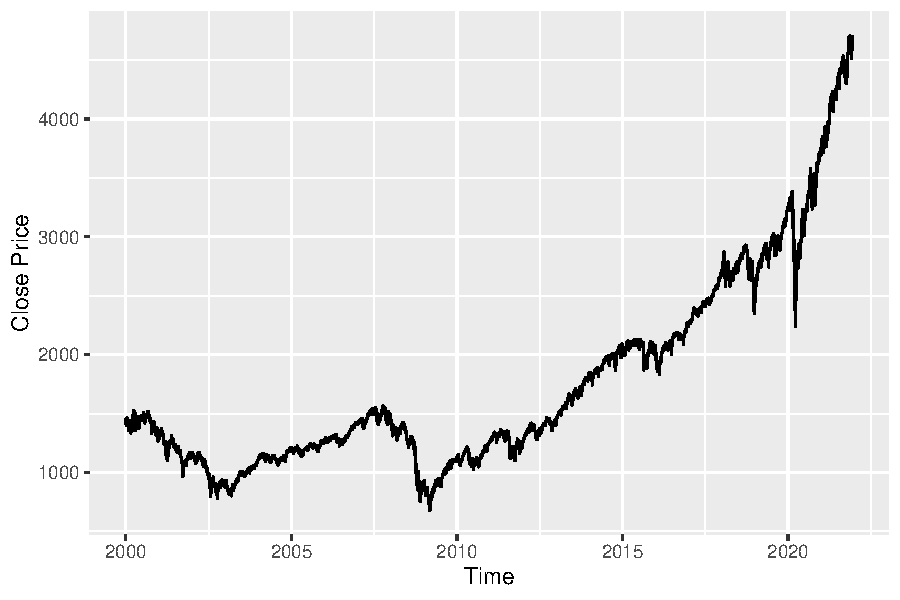
\includegraphics[scale=0.7]{fig/img/rawplotny.pdf}
    \caption{Daily Closing Value of S\&P-500 Index from 2000-01-30 to 2021-12-10.}
    \label{fig:rawplot}
\end{figure}
Clearly, this is a non-stationary time series with an upward trend abrupted by some periods with a spike in volatility. Testing the null hypothesis of non-stationary of the time series using the augmented Dickey-Fuller test yields a p-value of 0.99, which clearly exceeds any reasonable significance level. Furthermore, plotting the process of log-returns $(R_{t})_{t=1}^{5521}$ clearly supports the first stylized fact of volatility clustering: 
\begin{figure}[H]\label{volahej}
    \centering
    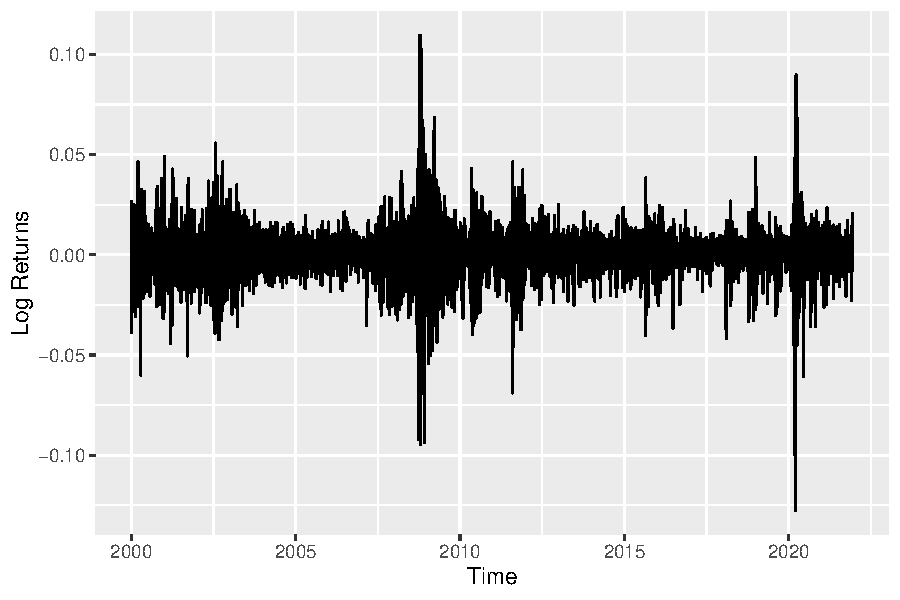
\includegraphics[scale=0.7]{fig/img/log-return-ny.pdf}
    \caption{Log-Returns of the S\&P-500 Index from 2000-01-03 to 2021-12-10.}
    \label{fig:plot2}
\end{figure}
Volatility clustering is clear, especially in the time periods surrounding the financial crisis of 2008, and the emergence of COVID-19 in 2020, both of which generated a great amount of disturbance in the financial markets. Since the log-returns time series $(R_{t})_{t=1}^{5521}$ in Figure 2.2 resembles a white noise process with volatility spikes, we expect the corresponding correlogram to show no significant autocorrelation in the log-returns. Plotting the sample autocorrelation $\hat{\rho}_{R}$ along with the confidence bands of $\pm \Phi^{-1}(1-\alpha/2)/\sqrt{n}$, where $\Phi^{-1}:[0,1]\to \R$ is the quantile function of the standard normal distribution, yields Figure 2.3.
\begin{figure}[H]
    \centering
    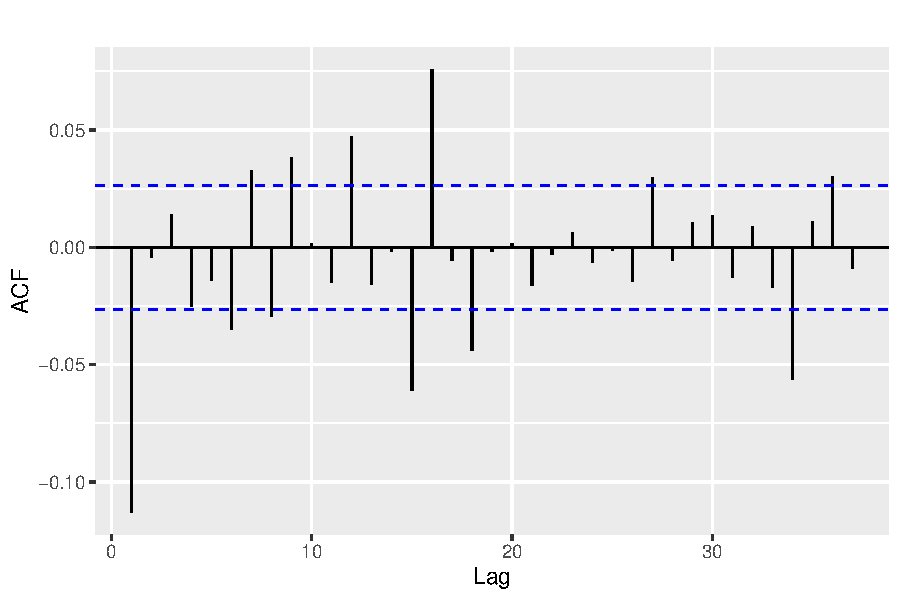
\includegraphics[scale=0.7]{fig/img/nytacfplotwuhuuu.pdf}
    \caption{Correlogram of the Log-Return Time Series.}
    \label{fig:my_label}
\end{figure}
Please note that for the given plot, we have chosen a significance level of $\alpha=0.05$ \textcolor{red}{and the number of observations is $n=5521$.} It is clear that for all lags greater than 2, there is no significant autocorrelation in the return process, since most correlations are bounded by the confidence bands with a few exceptions slightly rising above the bands. We can formally test whether these autocorrelations are significant or not using the Ljung-Box test. Testing the null hypothesis of independence on the log-returns using the Ljung-Box Q-statistic \eqref{eq:lb-qts} yields the following p-values: 
\begin{figure}[H]
    \centering
    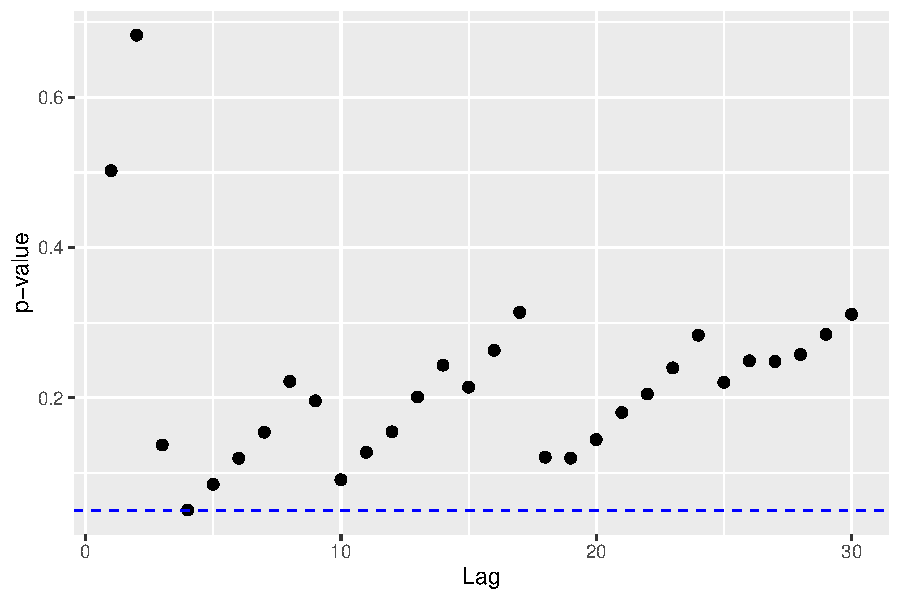
\includegraphics[scale=0.7]{fig/img/ny_ljnugbox_ggplot.pdf}
    \caption{P-values for the Ljung-Box Q-Statistic.}
    \label{fig:ljungbox}
\end{figure}
%\textcolor{red}{Det her plot er kun for de første 90 observationer af log-return serien.} 
The plot of p-values shows that at none of the first 30 lags is it possible to reject the null hypotheis of independence.
%Testing the null hypothesis of independence, and thus also whether the given ACF-values are uncorrelated, yields a p-value of 0.98. 
%This clearly exceeds any reasonable significance level, and thus we cannot reject the null hypothesis of independence.
Thus, we accept the log-returns as being independent, and hence by implication, they are also uncorrelated. 

Proceeding accordingly, the correlogram of the processes $(|R_{t}|)_{t=1}^{5521}$ and $(R_{t}^{2})_{t=1}^{5521}$ are plotted in the following Figure 2.5 and Figure 2.6 respectively:
\begin{figure}[H]
\begin{minipage}[b]{0.45\linewidth}
\centering
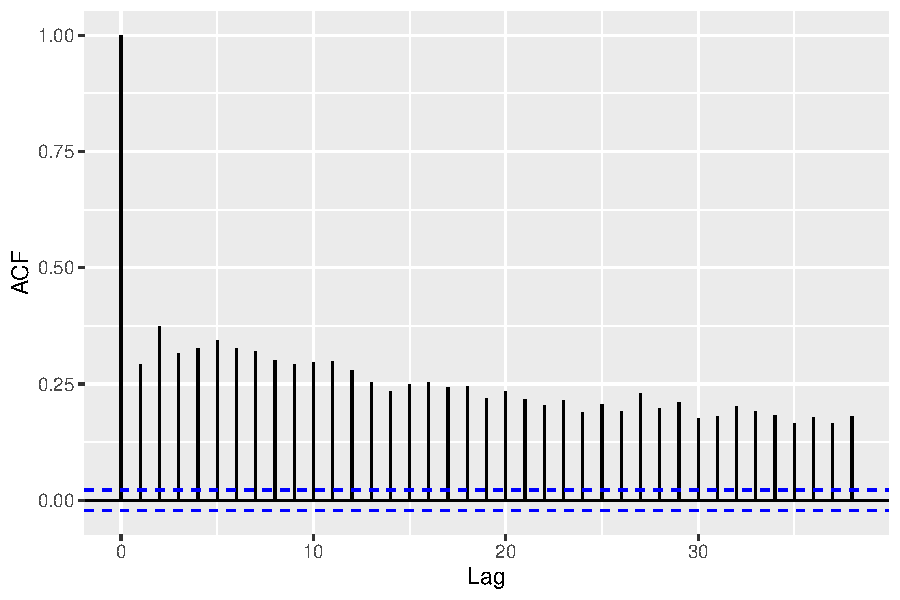
\includegraphics[width=1.2\linewidth, height=0.3\textheight]{fig/img/acfabsret.pdf}
\caption{Correlogram of $(|R_{t}|)_{t=1}^{5521}$.}
\label{fig:ACF1}
\end{minipage}
\hspace{0.7cm}
\begin{minipage}[b]{0.45\linewidth}
\centering
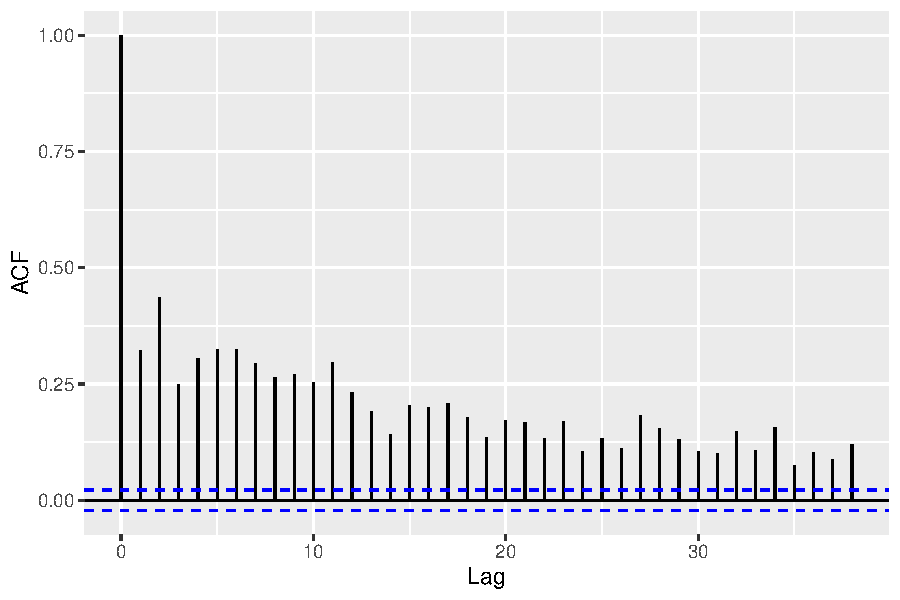
\includegraphics[width=1.2\linewidth, height=0.3\textheight]{fig/img/acfsquaredret.pdf}
\caption{Correlogram of $(R_{t}^{2})_{t=1}^{5521}$.}
\label{fig:ACF2}
\end{minipage}
\end{figure}
Evidently, there is strong autocorrelation in the processes of absolute and squared log-returns for all lags greater than 1. Thus, we now turn to the third stylized fact, which addresses whether the empirical distribution of $R$ is leptokurtic. Comparing the sample quantiles against the quantiles of a normal distribution gives the following QQ-plot:\vspace{-6 pt}
\begin{figure}[H]
    \centering
    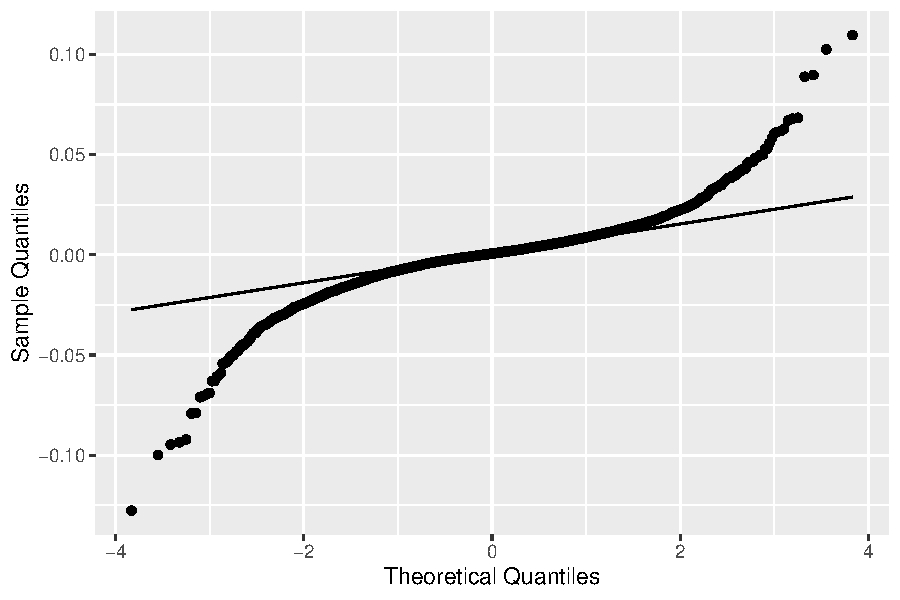
\includegraphics[scale=0.7]{fig/img/qqplot.pdf}
    \caption{QQ-Plot of Sample Quantiles against Normal Quantiles.}
    \label{fig:qqplot1}
\end{figure}
The return process is visibly much more heavy-tailed than the normal distribution with much more probability mass condensed at the tails. Furthermore, the empirical histogram $H_{R}:\R\to [0,\infty)$ of the return process $R$ with fineness of partition $k$ is then given by:
\begin{equation}
    H_{R}(x)=\frac{2^{k}}{N}\sum_{i=1}^{N}\ind_{\left(\frac{j_{k}(x)-1}{2^{k}},\frac{j_{k}(x)}{2^{k}}\right]}(R_{i}),
\end{equation}
where $N$ is the number of observations in our return process, and $j_{k}(x)\coloneqq [2^{k}x]$ for $x\in \R$. We can plot this function $H_{R}$ along with the normal density $f\sim \mathcal{N}(\mu,\sigma^{2})$, where the parameter $\mu$ is chosen as the mean of the return process, and $\sigma$ is similarly the standard deviation of the return process. Additionally, the non-parametric kernel density estimate of the return process is drawn in blue. The resulting plot is then:
\begin{figure}[H]
    \centering
    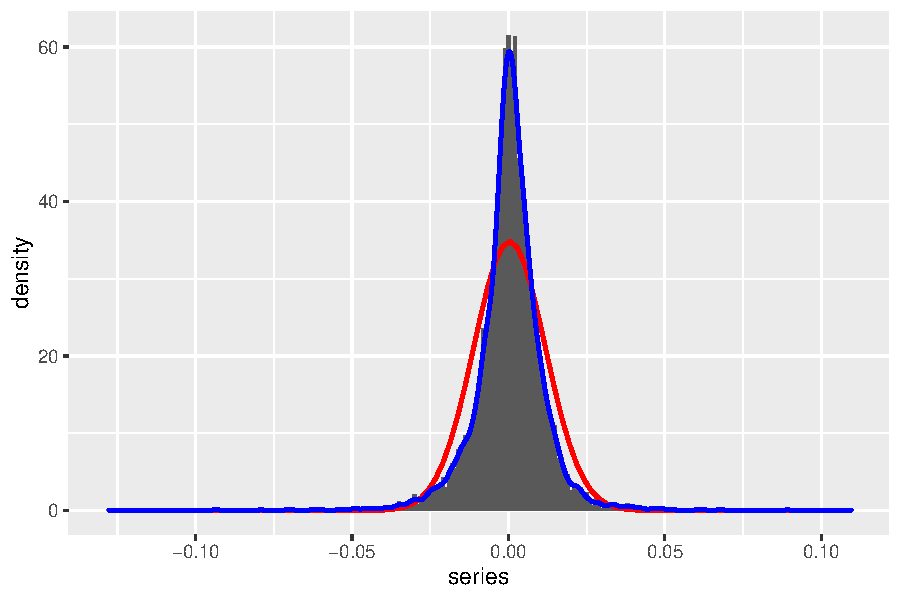
\includegraphics[scale=0.75]{fig/img/histogramplot.pdf}
    \caption{Empirical Histogram with Theoretical Normal Density and Estimated Density.}
    \label{fig:my_label}
\end{figure}
Evidently, the empirical distribution of the log-returns is more sharply spiked at the center than the corresponding normal density drawn in red. Similarly, the kernel density decays more slowly than exponentially, indicating that the empirical distribution is leptokurtic. Calculating the sample kurtosis of the log-returns series confirms this, yielding a kurtosis coefficient of 14.07, which is significantly above the mesokurtic level of 3.

Turning to the final stylized fact concerning the leverage effect, we can check how the time series $R^{+}_{t}\coloneqq \max\{ R_{t},0\}$ and $R^{-}_{t}\coloneqq \min\{-R_{t},0\}$ are correlated with the absolute returns $|R_{t}|$. As indicated by Figure 2.9, there is strong cross-correlation between $|R_{t}|$ and $R^{+}_{t}$ with all lags rising above the confidence bands. However, there is even stronger cross-correlation between $|R_{t}|$ and $R^{-}_{t}$, especially for positive lags, which rise significantly above $0.2$. Hence, Figure 2.10 supports the presence of the leverage effect in the data, indicating that market volatility increases more, when returns are negative.
%The observations of $|R_{t}|$ and $R^{+}_{t}$ are approximately 54\% equal and conversely, we have that the observations of $|R_{t}|$ and $R^{-}_{t}$ are approximately 46\% equal.
\begin{figure}[H]
\begin{minipage}[b]{0.45\linewidth}
\centering
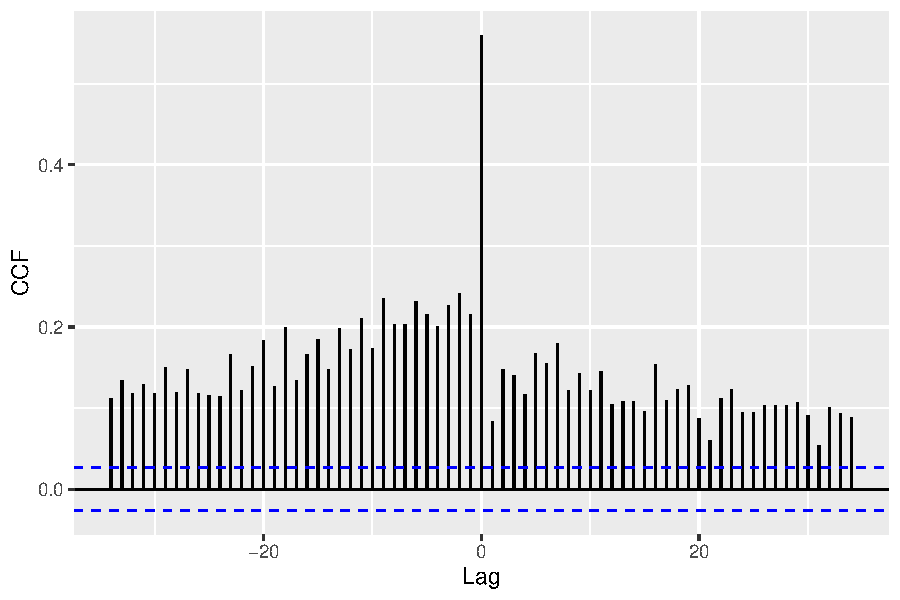
\includegraphics[width=1.2\linewidth, height=0.3\textheight]{fig/img/ccfmaxRny.pdf}
\caption{CCF of $|R_{t}|$ and $R^{+}_{t}$.}
\label{fig:ACF1}
\end{minipage}
\hspace{0.7cm}
\begin{minipage}[b]{0.45\linewidth}
\centering
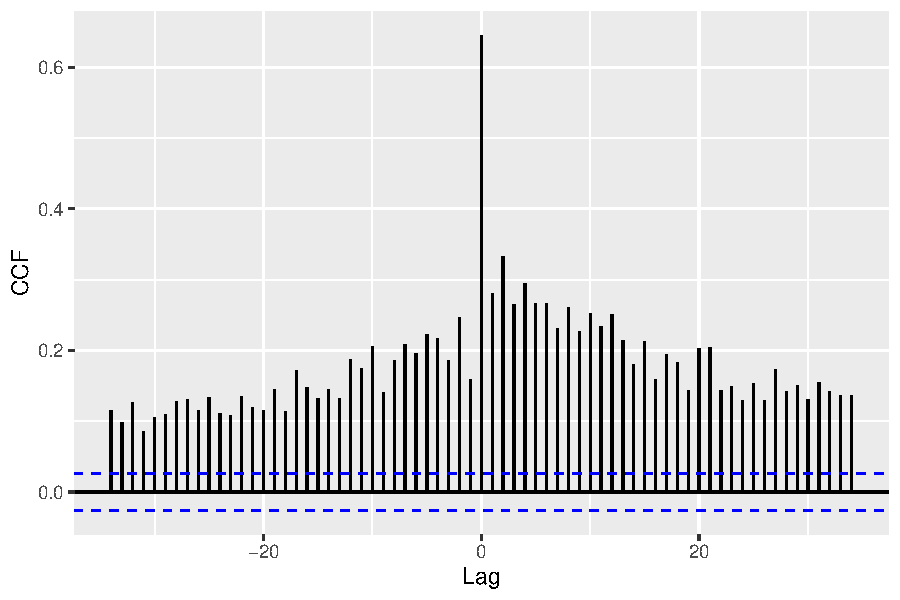
\includegraphics[width=1.2\linewidth, height=0.3\textheight]{fig/img/ccfminusR.pdf}
\caption{CCF of $|R_{t}|$ and $R^{-}_{t}$.}
\label{fig:ACF2}
\end{minipage}
\end{figure}
Generally, the cross-correlations are numerically large for both negative and positive lags, signifying that either series leads or lags the other. This comes as no surprise, since the two series have a vast overlap of observations. Approximately 54\% of the observations in $|R_{t}|$ and $R^{+}_{t}$ are equal, and conversely, we have that approximately 46\% of the observations in $|R_{t}|$ and $R^{-}_{t}$ are equal. 

\begin{table}[H]
\centering
\begin{tabular}{llllllll}
\hline
$h$ & 1 & 2 & 3 & 4 & 5 & 6 & 7 \\ \hline
$\hat{\rho}_{R}(h)$ & -0.1128 & -0.0043 & 0.0139 & -0.0252 & -0.0139 & -0.0351 & 0.0326 \\
$\hat{\rho}_{|R|}(h)$ & 0.3078 & 0.4033 & 0.3395 & 0.3458 & 0.3616 & 0.3523 & 0.3412\\
$\hat{\rho}\left(R^{+}_{t-h},|R_{t}|\right)$ & 0.0839 & 0.1473 & 0.1404 & 0.1164 & 0.1675 & 0.1554 & 0.1791\\ 
$\hat{\rho}\left(R^{-}_{t-h},|R_{t}|\right)$ & 0.2801 & 0.3326 & 0.2649 & 0.2942 & 0.2655 & 0.2659 & 0.2311 \\ \hline
\end{tabular}
\end{table}
%Specifically, it will be checked if the empirical distribution of log-returns is leptokurtic, if there is significant autocorrelation in absolute log-returns, and if there is significant autocorrelation in squared log-returns. The dataset to be utilized is the S\&P-500 index. We have chosen the daily closing value of the index in the time span 2006-MM-DD to 2021-MM-DD.

%The results of the

\newpage
\section{Empirical Results}
This section aims to discuss the empirical results of modelling the log-returns of the daily closing price for the S\&P 500 stock market index under the GARCH framework using the \code{R} software package \code{rugarch}. The full-sample of our data starts from the $3$rd of January $2000$ to the 10th of December 2021 spanning a $21$ year period. This full-sample is split into an in-sample and out-of-sample period with the 30th of April 2021 being the splitting date. First, a short introduction to the \code{rugarch} package is provided. Then, the resulting in-sample parameter estimation and model diagnostics are presented. Lastly, the out-of-sample forecasting performance of a select few models is evaluated using the Diebold-Mariano test.

\subsection{A Short Introduction to the \code{rugarch} Package in \code{R}*}\label{ss:intro-rugarch}
The \code{rugarch} software package in \code{R} implements the previously discussed GARCH estimation and forecasting procedures. The implementation uses three functions as its main interface.

The \code{ugarchfit} function is used to fit a GARCH model. The specification of the GARCH model to be fitted is defined via a call to the \code{ugarchspec} function. Then, forecasts from the fitted model are obtained using the \code{ugarchforecast} function via a call to the \code{ugarchfit} function. An example of their usage is shown underneath.
\lstinputlisting{code/exampleone.R}
Here \code{variance.model} is a list specifying the type of GARCH model and its order, \code{distribution.model} specifies the error distribution, \code{mean.model} is a list of the mean model specification, \code{solver} specifies the numerical optimization technique used to maximize \eqref{eq:garch-mle}, \code{out.sample} specifies the number of data points from the end to withhold for out-of-sample forecasting later, and \code{n.ahead} specifies the forecast horizon.

Please note that, in this project report, the mean model is always specified, as in the example above, to be constantly equal to zero in compliance with the assumption made in Section \ref{sec:gf}. Moreover, the \code{hybrid} strategy solver ...

%The \code{ugarchforecast} function implements forecasting given a fitted GARCH model via a call to the \code{ugarchfit} function. An example is shown underneath. %Note that \code{ugarchforecast} can also be used via a secondary dispatch method by calling \code{ugarchspec}. However, we do not make use of this secondary dispatch method, and therefore, the interested reader is referred to the references listed at the beginning of this chapter for more details.
%\lstinputlisting{code/exampleone-continued.R}
%Here \code{n.ahead} specifies the forecast horizon, that is, 


\subsection{In-sample Model Selection and Diagnostics}
Now, using the \code{rugarch} software package in \code{R}, each GARCH model discussed in the first chapter of this project report is fitted to the in-sample log-returns of the daily closing price for the S\&P 500 index. The results are shown in in Table \ref{tab:insample-res}. 

Note that the order of a particular GARCH model, displayed in brackets below an information criterion value, is chosen such that it minimizes that particular information criterion. A notable finding is that ...

Also, the results of the diagnostics tests applied to the residuals of each GARCH model is given in Appendix \ref{}. Some notable findings are...

\newpage
\begin{table}[H]
\centering
\begin{adjustbox}{angle=90}
\begin{tabular}{llllllllllllllllllllllllll}
\hline
Model & \multicolumn{3}{c}{GARCH} & \multicolumn{3}{c}{EGARCH} & \multicolumn{3}{c}{TGARCH} & \multicolumn{3}{c}{AVGARCH} & \multicolumn{3}{c}{GJR-GARCH} & \multicolumn{3}{c}{APGARCH} \\ \hline
Distribution       & norm & std & ged & norm & std & ged & norm & std & ged & norm & sted & ged & norm & sted & ged & norm & std & ged  \\
AIC                &  &  &  &  &  &  &  &  &  &  &  &  &  &  &  &  &  & \\
BIC                &  &  &  &  &  &  &  &  &  &  &  &  &  &  &  &  &  & \\
HQIC               &  &  &  &  &  &  &  &  &  &  &  &  &  &  &  &  &  & \\
SIC                &  &  &  &  &  &  &  &  &  &  &  &  &  &  &  &  &  & \\
Log-Likelihood     &  &  &  &  &  &  &  &  &  &  &  &  &  &  &  &  &  & \\
Ljung-Box Test     &  &  &  &  &  &  &  &  &  &  &  &  &  &  &  &  &  & \\
LM test            &  &  &  &  &  &  &  &  &  &  &  &  &  &  &  &  &  & \\ \hline
\end{tabular}
\end{adjustbox}
\caption{Suck My P33 P33}
\label{tab:insample-res}
\end{table}


%The implementation of the in-sample estimation is done such that one has to choose the maximal orders $p$ and $q$ of the GARCH models to be estimated. Furthermore, one has to choose between the specifications \code{sGARCH} (a standard GARCH model), \code{eGARCH}, \code{TGARCH}, \code{gjrGARCH}, \code{apARCH}, and \code{AVGARCH}, which have all been presented in Section 2.3. Finally, one also the conditional distribution of the model, which can be specified as a normal distribution, a Student's t-distribution, and a generalized error distribution as discussed in  Section 2.3.2. For instance, if one wants to fit models of maximal orders $p=q=2$ with specifications \code{sGARCH}, \code{eGARCH}, and \code{TGARCH}, and all 3 conditional distributions, then one has to fit a total of $8\cdot 3\cdot 3=72$ models. In fact, there are a total of $9$ combinations of the orders, but the pathology $p=q=0$ has been exclude from the estimation procedure.

\newpage
\subsection{Out-of-sample Forecast Evaluation}\label{ss:app-oos-forecast}
This subsection first describes the recursive forecasting method used to conduct an out-of-sample forecasting performance comparison of the models discussed in the previous subsection. This out-of-sample forecasting performance is evaluated using the Diebold-Mariano test, described in Subsection \ref{ss:evf-dm}, which warrants a discussion of volatility proxies. At last, the results of this out-of-sample forecasting performance comparison are presented.

\subsubsection{Recursive Forecasting Method}
Once an appropriate GARCH model, fitted to the in-sample data, has been chosen by the minimization of some information criterion, it is possible to test the forecasting performance on the remaining data not used for estimation. Suppose our in-sample data is given by $(D_{t})_{t=1}^{T}$, where $T>1$ denotes the final time point in the sample. Furthermore, suppose that our forecasting horizon \code{n.ahead} is given by some $n\in \N$. Initially, we fit the model using our in-sample data, and use this fitted model to forecast the next $n$ time points. Then iteratively, the model is refit by augmenting our in-sample data with the point at $T+1$, and using this refitted model, we forecast ahead $n$ time points. If we have $m$ time points in our out-of-sample data, then naturally this procedure can only be done $m/n$ times.
%This is done using a recursive forecasting method, which for each time point in our out-of-sample data uses the fitted model to forecast the next \code{n.ahead} values. Then the model is re-fitted by augmenting our in-sample data with the next data point in the time series. Using this newly fitted model, the forecasting procedure is repeated, and the next \code{n.ahead} values are forecasted. The forecasting is done using \code{rugarchforecast}, which can both forecast the $\sigma_{t}^{2}$ series and the actual series. An example of 
%and then the forecasting procedure is repeated once again, and the next \code{n.ahead} values are forecasted. 

\subsubsection{Volatility Proxies}
For the subsequent discussion, let $R_{\leq T}=(R_{t})_{t=1}^{T}$, $T\in\Z$, denote a sample from a stochastic process of log-returns $R=(R_{t})_{t\in\Z}$, that is, $R_{t}=\log(P_{t}/P_{t-1})$, where $(P_{t})_{t\in\Z}$ is a stochastic process of daily prices for some financial asset. Assume that $R$ follows some GARCH process driven by $Z=(Z_{t})_{t\in\Z}$.

Recall that a volatility proxy must be specified to conduct a Diebold-Mariano test, see \eqref{eq:forecasterror}. In what follows, different volatility proxies are presented. A simple volatility proxy is the squared log-returns $R_{t}^{2}$. The motivation for using $R_{t}^{2}$ as a volatility is given by (b) in Proposition \ref{prop:rvmfacts}. However, it is important to note that $R_{t}^{2}$ is a noisy volatility proxy since from \eqref{eq:rvmkurtosis} and (d) in Proposition \ref{prop:rvmfacts}, it follows that:
\begin{equation*}
    \mathrm{Var}(R_{t}^{2})=\mathbb{E}[\sigma_{t}^{4}]\left(\kappa(Z_{t})-1\right).
\end{equation*}
Interpreting the results of the Diebold-Mariano test conducted using a noisy volatility proxy is \textcolor{red}{evidently problematic}, whence a less noisy volatility proxy is introduced next. This volatility proxy is applicable provided that high-frequency intradata is available. Let $R_{t,i,m}$ denote the intraday log-returns over a time interval $1/m$ on day $t$, that is:
\begin{equation*}
    R_{t,i,m}\coloneqq\log\left(\frac{P_{t-i/m}}{P_{t-(i-1)/m}}\right),\quad i\in\{1,\dots,m\},\hspace{4pt}m\in\N.
\end{equation*}
Notice that:
\begin{equation*}
    R_{t}=\sum_{i=1}^{m}R_{t,i,m}.
\end{equation*}
In regards to intraday log-returns, it is often reasonable to make the following assumptions:
\begin{equation*}
    \mathbb{E}[R_{t,i,m}\mid R_{\leq t-1}]=0,\quad\mathrm{Cov}(R_{t,i,m},R_{t,j,m})=0,\hspace{6pt} i\neq j.
\end{equation*}
In particular, the latter assumption above implies that:
\begin{equation*}
    \sigma_{t}^{2}=\mathbb{E}[R_{t}^{2}\mid R_{\leq t-1}]%=\mathrm{Var}[\sum_{i=1}^{m}R_{t,i,m}\mid R_{\leq t-1}]=\sum_{i=1}^{m}\mathrm{Var}[R_{t,i,m}\mid R_{\leq t-1}]
    =\sum_{i=1}^{m}\mathbb{E}[R_{t,i,m}^{2}\mid R_{\leq t-1}].
\end{equation*}
This motivates defining the so-called realized volatility (at frequency $m$) as:
\begin{equation}
    \mathrm{RV}_{t}^{(m)}\coloneqq\sum_{i=1}^{m}R_{t,i,m}^{2},
\end{equation}
The realized volatility is a less noisy volatility proxy compared to the squared log-returns when $m$ is chosen moderately large. This is argued in \ref{} with $m=288$. %hansen2005
Moreover, under certain regularity conditions, the realized volatility is a consistent estimator of $\sigma_{t}^{2}$, that is:
\begin{equation*}
    \mathrm{RV}_{t}^{(m)}\overset{p}{\to}\sigma_{t}^{2}\quad\textrm{as}\quad m\to\infty.
\end{equation*}
For details the interested reader is referred to \ref{}. %andersen2003
In this project report, the realized volatility at a frequency of $m=288$ for the S\&P 500 index is obtained via \ref{}. %https://realized.oxford-man.ox.ac.uk/

Lastly, a volatility proxy is provided by the Chicago Board Options Exchange (CBOE) volatility index (VIX). The CBOE VIX is a model-free measure of the expected volatility implied by the S\&P 500 index over the next 30 calender days. The details of how the VIX index is calculated is beyond the scope of this project report, the interested reader is referred to \ref{} for details. The data for the CBOE VIX is obtained via \ref{}. %https://finance.yahoo.com/quote/%5EVIX/

%Lastly, all the previously discussed volatility proxies are combined to form a new volatility proxy. This is done in the following manner: %\begin{equation}
%    s
%\end{equation}
%Here ...

\subsubsection{Results}







% Input files should be partitioned such that each file corresponds to one
% chapter. The \include command forces a page break and inserts the contents of
% the input file.

% \include{incl/main/example1}
% \include{incl/main/example2}
% ...

% Appendices are included inside an appendices block, which enumerates chapters
% with letters, starting from A, instead of numbers.
\begin{appendices}
  % \include{incl/app/appendix1}
  % \include{incl/app/appendix2}
  % ..
\end{appendices}

% The backmatter is for extra stuff. Headings are not numbered.
\backmatter

% Automatic list of references, based on which references in the literature
% database files were referenced throughout the document.
\bibliographystyle{apalike}
\bibliography{
  incl/bib/books,
  incl/bib/articles,
  incl/bib/software
}

\end{document}
